% Options for packages loaded elsewhere
% Options for packages loaded elsewhere
\PassOptionsToPackage{unicode}{hyperref}
\PassOptionsToPackage{hyphens}{url}
\PassOptionsToPackage{dvipsnames,svgnames,x11names}{xcolor}
%
\documentclass[
  10pt,
]{article}
\usepackage{xcolor}
\usepackage[margin=2cm]{geometry}
\usepackage{amsmath,amssymb}
\setcounter{secnumdepth}{5}
\usepackage{iftex}
\ifPDFTeX
  \usepackage[T1]{fontenc}
  \usepackage[utf8]{inputenc}
  \usepackage{textcomp} % provide euro and other symbols
\else % if luatex or xetex
  \usepackage{unicode-math} % this also loads fontspec
  \defaultfontfeatures{Scale=MatchLowercase}
  \defaultfontfeatures[\rmfamily]{Ligatures=TeX,Scale=1}
\fi
\usepackage{lmodern}
\ifPDFTeX\else
  % xetex/luatex font selection
\fi
% Use upquote if available, for straight quotes in verbatim environments
\IfFileExists{upquote.sty}{\usepackage{upquote}}{}
\IfFileExists{microtype.sty}{% use microtype if available
  \usepackage[]{microtype}
  \UseMicrotypeSet[protrusion]{basicmath} % disable protrusion for tt fonts
}{}
\makeatletter
\@ifundefined{KOMAClassName}{% if non-KOMA class
  \IfFileExists{parskip.sty}{%
    \usepackage{parskip}
  }{% else
    \setlength{\parindent}{0pt}
    \setlength{\parskip}{6pt plus 2pt minus 1pt}}
}{% if KOMA class
  \KOMAoptions{parskip=half}}
\makeatother
% Make \paragraph and \subparagraph free-standing
\makeatletter
\ifx\paragraph\undefined\else
  \let\oldparagraph\paragraph
  \renewcommand{\paragraph}{
    \@ifstar
      \xxxParagraphStar
      \xxxParagraphNoStar
  }
  \newcommand{\xxxParagraphStar}[1]{\oldparagraph*{#1}\mbox{}}
  \newcommand{\xxxParagraphNoStar}[1]{\oldparagraph{#1}\mbox{}}
\fi
\ifx\subparagraph\undefined\else
  \let\oldsubparagraph\subparagraph
  \renewcommand{\subparagraph}{
    \@ifstar
      \xxxSubParagraphStar
      \xxxSubParagraphNoStar
  }
  \newcommand{\xxxSubParagraphStar}[1]{\oldsubparagraph*{#1}\mbox{}}
  \newcommand{\xxxSubParagraphNoStar}[1]{\oldsubparagraph{#1}\mbox{}}
\fi
\makeatother

\usepackage{color}
\usepackage{fancyvrb}
\newcommand{\VerbBar}{|}
\newcommand{\VERB}{\Verb[commandchars=\\\{\}]}
\DefineVerbatimEnvironment{Highlighting}{Verbatim}{commandchars=\\\{\}}
% Add ',fontsize=\small' for more characters per line
\usepackage{framed}
\definecolor{shadecolor}{RGB}{241,243,245}
\newenvironment{Shaded}{\begin{snugshade}}{\end{snugshade}}
\newcommand{\AlertTok}[1]{\textcolor[rgb]{0.68,0.00,0.00}{#1}}
\newcommand{\AnnotationTok}[1]{\textcolor[rgb]{0.37,0.37,0.37}{#1}}
\newcommand{\AttributeTok}[1]{\textcolor[rgb]{0.40,0.45,0.13}{#1}}
\newcommand{\BaseNTok}[1]{\textcolor[rgb]{0.68,0.00,0.00}{#1}}
\newcommand{\BuiltInTok}[1]{\textcolor[rgb]{0.00,0.23,0.31}{#1}}
\newcommand{\CharTok}[1]{\textcolor[rgb]{0.13,0.47,0.30}{#1}}
\newcommand{\CommentTok}[1]{\textcolor[rgb]{0.37,0.37,0.37}{#1}}
\newcommand{\CommentVarTok}[1]{\textcolor[rgb]{0.37,0.37,0.37}{\textit{#1}}}
\newcommand{\ConstantTok}[1]{\textcolor[rgb]{0.56,0.35,0.01}{#1}}
\newcommand{\ControlFlowTok}[1]{\textcolor[rgb]{0.00,0.23,0.31}{\textbf{#1}}}
\newcommand{\DataTypeTok}[1]{\textcolor[rgb]{0.68,0.00,0.00}{#1}}
\newcommand{\DecValTok}[1]{\textcolor[rgb]{0.68,0.00,0.00}{#1}}
\newcommand{\DocumentationTok}[1]{\textcolor[rgb]{0.37,0.37,0.37}{\textit{#1}}}
\newcommand{\ErrorTok}[1]{\textcolor[rgb]{0.68,0.00,0.00}{#1}}
\newcommand{\ExtensionTok}[1]{\textcolor[rgb]{0.00,0.23,0.31}{#1}}
\newcommand{\FloatTok}[1]{\textcolor[rgb]{0.68,0.00,0.00}{#1}}
\newcommand{\FunctionTok}[1]{\textcolor[rgb]{0.28,0.35,0.67}{#1}}
\newcommand{\ImportTok}[1]{\textcolor[rgb]{0.00,0.46,0.62}{#1}}
\newcommand{\InformationTok}[1]{\textcolor[rgb]{0.37,0.37,0.37}{#1}}
\newcommand{\KeywordTok}[1]{\textcolor[rgb]{0.00,0.23,0.31}{\textbf{#1}}}
\newcommand{\NormalTok}[1]{\textcolor[rgb]{0.00,0.23,0.31}{#1}}
\newcommand{\OperatorTok}[1]{\textcolor[rgb]{0.37,0.37,0.37}{#1}}
\newcommand{\OtherTok}[1]{\textcolor[rgb]{0.00,0.23,0.31}{#1}}
\newcommand{\PreprocessorTok}[1]{\textcolor[rgb]{0.68,0.00,0.00}{#1}}
\newcommand{\RegionMarkerTok}[1]{\textcolor[rgb]{0.00,0.23,0.31}{#1}}
\newcommand{\SpecialCharTok}[1]{\textcolor[rgb]{0.37,0.37,0.37}{#1}}
\newcommand{\SpecialStringTok}[1]{\textcolor[rgb]{0.13,0.47,0.30}{#1}}
\newcommand{\StringTok}[1]{\textcolor[rgb]{0.13,0.47,0.30}{#1}}
\newcommand{\VariableTok}[1]{\textcolor[rgb]{0.07,0.07,0.07}{#1}}
\newcommand{\VerbatimStringTok}[1]{\textcolor[rgb]{0.13,0.47,0.30}{#1}}
\newcommand{\WarningTok}[1]{\textcolor[rgb]{0.37,0.37,0.37}{\textit{#1}}}

\usepackage{longtable,booktabs,array}
\newcounter{none} % for unnumbered tables
\usepackage{calc} % for calculating minipage widths
% Correct order of tables after \paragraph or \subparagraph
\usepackage{etoolbox}
\makeatletter
\patchcmd\longtable{\par}{\if@noskipsec\mbox{}\fi\par}{}{}
\makeatother
% Allow footnotes in longtable head/foot
\IfFileExists{footnotehyper.sty}{\usepackage{footnotehyper}}{\usepackage{footnote}}
\makesavenoteenv{longtable}
\usepackage{graphicx}
\makeatletter
\newsavebox\pandoc@box
\newcommand*\pandocbounded[1]{% scales image to fit in text height/width
  \sbox\pandoc@box{#1}%
  \Gscale@div\@tempa{\textheight}{\dimexpr\ht\pandoc@box+\dp\pandoc@box\relax}%
  \Gscale@div\@tempb{\linewidth}{\wd\pandoc@box}%
  \ifdim\@tempb\p@<\@tempa\p@\let\@tempa\@tempb\fi% select the smaller of both
  \ifdim\@tempa\p@<\p@\scalebox{\@tempa}{\usebox\pandoc@box}%
  \else\usebox{\pandoc@box}%
  \fi%
}
% Set default figure placement to htbp
\def\fps@figure{htbp}
\makeatother





\setlength{\emergencystretch}{3em} % prevent overfull lines

\providecommand{\tightlist}{%
  \setlength{\itemsep}{0pt}\setlength{\parskip}{0pt}}



 


\usepackage{graphicx}
\usepackage{amsmath}
\usepackage{booktabs}
\usepackage{float}
\usepackage{caption}
\usepackage{setspace}
\usepackage{fancyhdr}
\captionsetup{font=small}
\singlespacing
\pagestyle{fancy}
\fancyhf{}
\fancyfoot[C]{\thepage}
\makeatletter
\@ifpackageloaded{caption}{}{\usepackage{caption}}
\AtBeginDocument{%
\ifdefined\contentsname
  \renewcommand*\contentsname{Table of contents}
\else
  \newcommand\contentsname{Table of contents}
\fi
\ifdefined\listfigurename
  \renewcommand*\listfigurename{List of Figures}
\else
  \newcommand\listfigurename{List of Figures}
\fi
\ifdefined\listtablename
  \renewcommand*\listtablename{List of Tables}
\else
  \newcommand\listtablename{List of Tables}
\fi
\ifdefined\figurename
  \renewcommand*\figurename{Figure}
\else
  \newcommand\figurename{Figure}
\fi
\ifdefined\tablename
  \renewcommand*\tablename{Table}
\else
  \newcommand\tablename{Table}
\fi
}
\@ifpackageloaded{float}{}{\usepackage{float}}
\floatstyle{ruled}
\@ifundefined{c@chapter}{\newfloat{codelisting}{h}{lop}}{\newfloat{codelisting}{h}{lop}[chapter]}
\floatname{codelisting}{Listing}
\newcommand*\listoflistings{\listof{codelisting}{List of Listings}}
\makeatother
\makeatletter
\makeatother
\makeatletter
\@ifpackageloaded{caption}{}{\usepackage{caption}}
\@ifpackageloaded{subcaption}{}{\usepackage{subcaption}}
\makeatother
\usepackage{bookmark}
\IfFileExists{xurl.sty}{\usepackage{xurl}}{} % add URL line breaks if available
\urlstyle{same}
\hypersetup{
  pdftitle={Proyecto Final},
  pdfauthor={Ismael Maximiliano De Los Santos Huesca},
  colorlinks=true,
  linkcolor={blue},
  filecolor={Maroon},
  citecolor={Blue},
  urlcolor={Blue},
  pdfcreator={LaTeX via pandoc}}


\title{Proyecto Final}
\author{Ismael Maximiliano De Los Santos Huesca}
\date{2026-05-30}
\begin{document}
\maketitle

\begin{titlepage}

    % Logos alineados izquierda y derecha
    \begin{minipage}{0.45\textwidth}
        \raggedright
        
\includegraphics[width=7cm]{Logo_UNAM.png}
    \end{minipage}
    \hfill
    \begin{minipage}{0.45\textwidth}
        \raggedleft
        
\includegraphics[width=3.4cm]{Logo_LCG.png}
    \end{minipage}

    \centering
    \vspace*{2cm}

    {\Huge\bfseries Enriquecimiento funcional \par}
    \vspace{2cm}
    
    {\Large Transciptomica \par}
    \vspace{1cm}
    
    {\Large De Los Santos Huesca Ismael Maximiliano \par}
    \vspace{1cm}

    {\Large Dr. David Valle\par}
    \vspace{1cm}
    
    {\Large Fecha: 19 Mayo 2026 \par}
    
    \vfill

\end{titlepage}

\renewcommand*\contentsname{Table of Contents}
{
\setcounter{tocdepth}{3}
\tableofcontents
}

\newpage

\begin{Shaded}
\begin{Highlighting}[]
\NormalTok{\#| echo: false }
\NormalTok{\#| warning: false}
\NormalTok{\#| message: false}
\NormalTok{\#R envirorment}
\NormalTok{.libPaths("/export/space3/users/ismadlsh/conda/envs/rnaseq\_r/lib/R/library")}

\NormalTok{\#chargue all the libraries needed for DEA}
\NormalTok{library(DESeq2)}
\NormalTok{library(ggplot2)}
\NormalTok{library(ComplexHeatmap)}
\NormalTok{library(dplyr)}
\NormalTok{library(tibble)}
\NormalTok{library(edgeR)}
\NormalTok{library(knitr)}
\NormalTok{library(tidyr)}
\NormalTok{library(kableExtra)}
\NormalTok{library(variancePartition)}
\NormalTok{library(R6)}
\NormalTok{library(gridExtra)}
\NormalTok{library(grid)}
\end{Highlighting}
\end{Shaded}

\section{Introducción}\label{introducciuxf3n}

El cerebro es probablemente el órgano más complejo con el que contamos
los seres humanos, esto implica un mayor número de tipos celulares
neuronales que se especializan en distintas funciones fisiológicas en
diferentes estructuras cerebrales como el hipotálamo
\hyperref[section]{1}. Así mismo, dentro del linaje neuronal las
neuronas efectoras de señales como tal no son los únicos tipos
importantes para el correcto funcionamiento de este tejido, pues células
como las pertenecientes a la glía son fundamentales en muchos procesos
tanto homeostáticos como de soporte, plasticidad y protección
\hyperref[section-1]{2}.

Particularmente, los astrocitos son células gliales que participan en el
mantenimiento homeostático, modulación y creación de sinapsis,
regulación y soporte de las células neuronales; sin embargo,
recientemente se ha señalado su papel en procesos como la inflamación,
teniendo fenotipos específicos de respuesta a estas perturbaciones y en
función de su interacción con la microglía \hyperref[section-2]{3}. Esto
provoca la disrupción de funciones basales de estas células, limitando
su capacidad de sostenimiento para las neuronas e incluso causando
citotoxicidad.

De esta forma, resulta relevante explorar los mecanismos que influencian
los procesos neuroinflamatorios y afectan la homeostasis de estas
células, cuyos fenotipos activados y neurotóxicos se encuentran
asociados a enfermedades neurodegenerativas como el Alzheimer
\hyperref[section-3]{4}. Un estudio reciente explora la influencia de la
dependencia al alcohol (etanol, EtOH) en ratones
\emph{Aldh1l1-eGFP/Rpl10a} \hyperref[section-4]{5}. En el mismo se
genera una dependencia a esta sustancia mediante la ingesta constante de
los individuos para analizar las muestras extraídas del núcleo accumbens
(NAc) y observar las muestras generales dentro del tejido cerebral y
particularmente de las células astrocíticas, para las cuales utilizan
\textbf{TRAP} (\emph{translating ribosome affinity purification},
muestras IP) y de esta forma aislar solamente los ácidos nucleicos de
los astrocitos.

\subsection{Planteamiento}\label{planteamiento}

Con el fin de estudiar las diferencias transcripcionales entre las
condiciones \emph{Dependent} (ratones consumidores de alcohol) y
\emph{Naive} (sin consumo de alcohol), se seleccionaron 6 réplicas
biológicas de cada condición bajo el identificador de acceso GEO
\texttt{GSE308880} que hubieran sido procesadas en el mismo lote y con
una distribución de sexos lo más uniforme posible para considerarse
posteriormente en el análisis.

\begin{table}[htbp]
\centering
\scriptsize
\resizebox{\textwidth}{!}{%
\begin{tabular}{lrlllll}
\hline
 Run         &      Bases & batch   & Experiment   & Fraction   & sex    & treatment   \\
\hline
 SRR35568686 & 7056141000 & L       & SRX30641926  & IP         & female & Dependent   \\
 SRR35568638 & 6422935500 & L       & SRX30641950  & IP         & female & Dependent   \\
 SRR35568687 & 7195563300 & L       & SRX30641926  & IP         & female & Dependent   \\
 SRR35568639 & 6567543300 & L       & SRX30641950  & IP         & female & Dependent   \\
 SRR35568650 & 8408655900 & L       & SRX30641944  & IP         & male   & Dependent   \\
 SRR35568651 & 8532258900 & L       & SRX30641944  & IP         & male   & Dependent   \\
 SRR35568623 & 6641559600 & L       & SRX30641958  & IP         & female & Naïve       \\
 SRR35568626 & 7019469600 & L       & SRX30641956  & IP         & male   & Naïve       \\
 SRR35568627 & 7132121400 & L       & SRX30641956  & IP         & male   & Naïve       \\
 SRR35568631 & 7998479400 & L       & SRX30641954  & IP         & male   & Naïve       \\
 SRR35568622 & 6489525000 & L       & SRX30641958  & IP         & female & Naïve       \\
 SRR35568634 & 7475442300 & L       & SRX30641952  & IP         & female & Naïve       \\
\hline
\end{tabular}
}
\caption{Tabla de metadatos estudio GSE308880, muestras seleccionadas}
\end{table}

Con el objetivo de evaluar estas diferencias se llevó a cabo un análisis
de expresión diferencial (DEA) entre ambas condiciones. Para ello, se
realizó la descarga de los datos de secuenciación a través de los
identificadores únicos de \emph{Short Read Run} (SRR) mediante
\texttt{fasterq-dump} \hyperref[section-5]{6}. Asimismo, se utilizaron
herramientas de limpieza de archivos de secuenciación como
\texttt{fastp} {[}7{]}, cuyos parámetros de limpieza fueron definidos a
partir de los reportes de control de calidad generados con
\texttt{FastQC} {[}8{]} y \texttt{MultiQC} {[}9{]}. Con las secuencias
limpias se procedió al alineamiento mediante las herramientas
\texttt{STAR} {[}10{]} y \texttt{HISAT2} {[}11{]}, dos alineadores
tradicionales seleccionados con el objetivo de evaluar su desempeño, ya
que se ha demostrado que la elección de la herramienta de alineación no
solo es fundamental para los pasos posteriores, sino que también es
dependiente de los datos analizados. Posteriormente, y de acuerdo con la
elección de los alineadores, se realizó la cuantificación mediante
\texttt{featureCounts} {[}12{]} para obtener las matrices de conteo y
finalmente proceder con todo el análisis de expresión diferencial
utilizando \texttt{DESeq2} {[}13{]} como herramienta principal para el
DEA, con apoyo de funciones de paquetes como \texttt{variancePartition}
{[}14{]}, \texttt{edgeR} {[}15{]} y \texttt{limma} {[}16{]}.

\section{Metodología}\label{metodologuxeda}

\subsection{Descarga de los datos y
QC}\label{descarga-de-los-datos-y-qc}

El primer paso para realizar el DEA es la obtención de todos los datos
necesarios para cada etapa del análisis, desde los controles de calidad
(QC) y la limpieza de las secuencias, hasta la cuantificación de los
conteos y el análisis estadístico. Para ello fueron requeridos los
siguientes archivos:

\begin{itemize}
\tightlist
\item
  Genoma de referencia en formato FASTA para el alineamiento: se utilizó
  la misma versión del genoma de referencia de \emph{Mus musculus},
  \texttt{GRCm39}, pero en su última \emph{release} (M38), incluyendo
  todas las secuencias (\texttt{ALL}) del genoma completo {[}17{]}, a
  diferencia de la versión M28 utilizada en el estudio original.
\item
  Archivo de anotación: se seleccionó el archivo \emph{Comprehensive
  gene annotation} para todas las secuencias (\texttt{ALL})
  correspondiente a la misma versión y \emph{release}
  (\texttt{GRCm39\ M38}).
\end{itemize}

\begin{quote}
Estos archivos fueron descargados mediante los enlaces SFTP de GENCODE
utilizando el comando \texttt{wget} (command run 1).
\end{quote}

\begin{itemize}
\tightlist
\item
  Tabla de metadatos de las muestras: obtenida directamente del
  \emph{Run Selector} asociado al identificador GEO
  \href{https://www.ncbi.nlm.nih.gov/geo/query/acc.cgi?acc=GSE308880}{GSE308880}.
\item
  Archivos de secuenciación: todos los correspondientes a las
  condiciones de interés fueron descargados a través de los
  identificadores SRR presentes en la tabla de metadatos.
\end{itemize}

Para el proceso de descarga y control de calidad (QC) se desarrolló un
\emph{pipeline} en Nextflow que permite realizar ambas tareas
simultáneamente (\texttt{src/preprocces\_data.nf}) (command run 2).

Una vez descargados los datos, el QC reveló que las secuencias presentan
un \emph{Phred score} muy alto, lo que indica una alta confianza en la
identificación de bases y, en general, una buena distribución en las
métricas relacionadas con la calidad de la secuenciación. Esto sugiere
una reacción de secuenciación adecuada, observándose únicamente
advertencias (\emph{warnings}) en las secuencias 1 de cada par respecto
a la calidad por posición en el \emph{flowcell}. Dado que esta
advertencia fue uniforme entre las muestras, no representa una fuente
importante de sesgo.

Sin embargo, no todas las métricas fueron óptimas, por lo que se
procedió a la limpieza de las secuencias mediante el software
\texttt{fastp}, el cual permite corregir aquellas regiones que no
superan completamente el QC. En nuestros datos fue evidente la presencia
de adaptadores, particularmente aquellos enriquecidos en secuencias
repetitivas como PolyG y PolyA, así como un sesgo hacia bases T al
inicio de las lecturas. Por ello se ejecutó el siguiente paso del
\emph{pipeline} de Nextflow \texttt{src/preprocces\_data.nf},
especificando las opciones \textbf{--trim\_front 1} y
\textbf{--trim\_poly\_x} (command run 3).

Tras la limpieza de los datos se obtuvo un nuevo reporte de MultiQC con
mejores estadísticas. Se logró corregir parcialmente el principal
problema relacionado con la presencia de adaptadores, aunque
persistieron algunas excepciones en posiciones intermedias, manteniendo
al mismo tiempo la mayor parte de la longitud original de las
secuencias. Por su parte, el porcentaje de GC permaneció prácticamente
sin cambios, lo que podría sugerir contaminación en las secuencias,
aunque sin afectar significativamente los pasos posteriores. De forma
similar, la duplicación y la sobre-representación de secuencias no
fueron corregidas, ya que el objetivo principal del estudio es
identificar cambios en la expresión génica (Anexo QC results).

\subsection{Alineamiento}\label{alineamiento}

Para la etapa de alineamiento, la elección de la herramienta no es
absoluta, ya que depende de múltiples factores. Algunos de ellos están
relacionados con limitaciones técnicas menos controlables, como la
información disponible del organismo estudiado o los recursos
computacionales de almacenamiento, tiempo y procesamiento. Este último
factor es una de las principales razones por las que muchos análisis
optan por utilizar \textbf{\emph{pseudoalineadores}} como
\texttt{salmon} o \texttt{kallisto}.

Sin embargo, debido a que estas aproximaciones utilizan como referencia
los transcritos previamente anotados, el espacio de búsqueda se limita
considerablemente y la asignación de lecturas puede verse afectada por
la capacidad de la secuenciación para capturar isoformas específicas
registradas en la anotación.

Por ello, en este trabajo se utilizaron dos alineadores tradicionales
ampliamente empleados en la literatura. Por un lado, \texttt{HISAT2} es
reconocido por su bajo consumo de recursos computacionales y menor
tiempo de ejecución en comparación con otros alineadores tradicionales,
siendo una opción accesible para estudios de gran escala y mostrando un
buen desempeño en lecturas cortas {[}18{]}. Por otro lado, se utilizó
\texttt{STAR}, una herramienta destacada por su alta sensibilidad,
rendimiento y capacidad de mapeo único {[}19{]}.

A pesar de que \texttt{STAR} suele considerarse un claro
\emph{trade-off} entre costo computacional y rendimiento, el desempeño
real para obtener los mejores resultados continúa siendo dependiente del
contexto y de los datos analizados. Por ello, se evaluó el rendimiento
de ambas herramientas utilizando las secuencias previamente procesadas
con \texttt{fastp}. Para ello se utilizó el mismo \emph{pipeline}
empleado durante la limpieza y descarga, el cual integra ambas
herramientas para su comparación (command run 5).

\begin{figure}[H]

{\centering \pandocbounded{
\includegraphics[keepaspectratio,alt={Gráfico del porcentaje de lecturas alineadas contra el tiempo consumido}]{../results/alignments/stats/aligned_vs_time.png}}

}

\caption{Alignment\_performance\_aligned\_vs\_time}

\end{figure}%

Como puede observarse, y en contraste con lo reportado en parte de la
literatura, \texttt{HISAT2} presentó un menor tiempo de ejecución bajo
condiciones equivalentes de recursos computacionales. Es posible que
esta diferencia se deba a un menor consumo de memoria RAM en comparación
con \texttt{STAR}. Asimismo, \texttt{HISAT2} mostró un mayor porcentaje
de lecturas alineadas, lo que inicialmente lo posiciona como una
alternativa atractiva para análisis posteriores.

\begin{figure}[H]

{\centering \pandocbounded{
\includegraphics[keepaspectratio,alt={Gráfico del porcentaje de lecturas multimapeadas contra el número de lecturas no alineadas}]{../results/alignments/stats/aligned_vs_time.png}}

}

\caption{Alignment\_performance\_multimapped\_vs\_non\_aligned}

\end{figure}%

Sin embargo, a diferencia de lo que podría sugerir la Figura 1, el
desempeño de \texttt{HISAT2} no resulta tan claramente superior. El
porcentaje de lecturas multimapeadas fue considerablemente mayor que en
\texttt{STAR}, lo cual es consistente con la menor cantidad de lecturas
no alineadas observadas. Esto sugiere una mayor capacidad de
\texttt{HISAT2} para asignar lecturas ambiguas, mientras que
\texttt{STAR} tiende a descartar aquellas para las cuales no existe una
asignación suficientemente confiable.

No obstante, al contrastar el porcentaje total de lecturas alineadas con
el porcentaje de lecturas multimapeadas, puede observarse que la
fracción de lecturas alineadas de forma única continúa siendo superior
en \texttt{HISAT2}. Por ello, y con el objetivo de conservar la mayor
cantidad posible de información biológica, se decidió utilizar las
matrices generadas por \texttt{HISAT2} para los análisis posteriores.

\subsubsection{Cuantificación}\label{cuantificaciuxf3n}

El \emph{pipeline} utilizado para el alineamiento (command run 5)
implementa también la generación de matrices de conteo a partir de los
alineamientos obtenidos mediante \texttt{featureCounts}, herramienta
perteneciente al paquete \texttt{subread}. Para ello se empleó el
archivo de anotación descargado previamente (command run 1) junto con
los parámetros mínimos necesarios para su funcionamiento.

Se configuró la herramienta para excluir lecturas multimapeadas y
considerar todas las lecturas independientemente de su longitud, ya que
el análisis de QC mostró una distribución uniforme en este aspecto. Como
resultado, fue posible obtener las matrices de conteo correspondientes a
\texttt{HISAT2}
(\texttt{results/count\_matrixes/hisat\_countMatrix.txt}).

\begin{table}[htbp]
\centering
\scriptsize
\resizebox{\textwidth}{!}{%
\begin{tabular}{rrrrrrrrrrrr}
\hline
   Dependent\_4 &   Dependent\_3 &   Dependent\_1 &   Dependent\_2 &   Dependent\_6 &   Dependent\_5 &   Naive\_4 &   Naive\_5 &   Naive\_1 &   Naive\_6 &   Naive\_3 &   Naive\_2 \\
\hline
             0 &             0 &             0 &             0 &             0 &             0 &         0 &         0 &         0 &         0 &         0 &         0 \\
             0 &             0 &             0 &             0 &             0 &             0 &         0 &         0 &         0 &         0 &         0 &         0 \\
            22 &           201 &            16 &           140 &           111 &            84 &        18 &       107 &       119 &        34 &        14 &        66 \\
             0 &             0 &             0 &             0 &             8 &            34 &         0 &         0 &         0 &         0 &         0 &         0 \\
            25 &             8 &            46 &             6 &            32 &            24 &        21 &        26 &        10 &        24 &        36 &        22 \\
\hline
\end{tabular}
}
\caption{Matriz de conteos hisat2 limpia y con los nombres de las muestras srr asignados }
\end{table}

Con esta tabla de conteos se procedió al análisis de expresión
diferencial (DEA), para el cual se utilizó el lenguaje de programación
\textbf{R}, debido a que cuenta con todas las librerías necesarias para
llevar a cabo este tipo de análisis estadísticos y bioinformáticos.

\subsection{DEA}\label{dea}

Para este paso se utilizarán las matrices de conteos generadas, así como
la tabla de metadatos previamente depurada y el archivo
\emph{transcript-to-gene} (\textbf{t2g}) generado a partir del archivo
de anotación GTF (command run 6).

\begin{Shaded}
\begin{Highlighting}[]
\NormalTok{\#| warning: false}
\NormalTok{\#| message: false}
\NormalTok{\#| echo: false}
\NormalTok{\#================================================}
\NormalTok{\# Count matrix}
\NormalTok{\#================================================}
\NormalTok{hi\_sat\_count\_mtrx = read.csv(}
\NormalTok{  "../results/count\_matrixes/hisat\_countMatrix\_clean.csv",}
\NormalTok{  header = TRUE,}
\NormalTok{  row.names = 1}
\NormalTok{)}
\NormalTok{star\_count\_mtrx = read.csv(}
\NormalTok{  "../results/count\_matrixes/star\_countMatrix\_clean.csv",}
\NormalTok{  header = TRUE,}
\NormalTok{  row.names = 1}
\NormalTok{)}
\end{Highlighting}
\end{Shaded}

\begin{Shaded}
\begin{Highlighting}[]
\NormalTok{\#| warning: false}
\NormalTok{\#| message: false}
\NormalTok{\#| echo: false}
\NormalTok{\#================================================}
\NormalTok{\# metadata}
\NormalTok{\#================================================}
\NormalTok{metadata\_raw = read.csv(}
\NormalTok{  "../data/GSE308880\_eOH\_dependence\_metadata\_clean.csv",}
\NormalTok{  header = TRUE}
\NormalTok{)}
\NormalTok{metadata = data.frame(metadata\_raw[c("treatment", "sex")])}
\NormalTok{row.names(metadata) = metadata\_raw[, "sample\_id"]}
\NormalTok{metadata$treatment = as.factor(metadata$treatment)}
\NormalTok{metadata$sex = as.factor(metadata$sex)}

\NormalTok{\#check if the names are the same of the ones that are in the count matrix}
\NormalTok{if (all(rownames(metadata) == colnames(hi\_sat\_count\_mtrx))) \{}
\NormalTok{  print(paste(}
\NormalTok{    "Los nombres de los metadatos concuerdan con la matriz de conteos hisat"}
\NormalTok{  ))}
\NormalTok{\}}

\NormalTok{if (all(rownames(metadata) == colnames(star\_count\_mtrx))) \{}
\NormalTok{  print(paste(}
\NormalTok{    "Los nombres de los metadatos concuerdan con la matriz de conteos star"}
\NormalTok{  ))}
\NormalTok{\} else \{}
\NormalTok{  star\_count\_mtrx = star\_count\_mtrx[, rownames(metadata)]}
\NormalTok{\}}

\NormalTok{\#================================================}
\NormalTok{\# anotation transcript to gene}
\NormalTok{\#================================================}
\NormalTok{annotation\_t2g = read.csv(}
\NormalTok{  "../data/reference/GRCm39\_vM38\_mouse\_t2g.tsv",}
\NormalTok{  header = TRUE,}
\NormalTok{  row.names = 1,}
\NormalTok{  sep = "\textbackslash{}t"}
\NormalTok{)}
\NormalTok{\#mapper to define gene names}
\NormalTok{gene\_name\_map = annotation\_t2g["gene\_name"]}
\end{Highlighting}
\end{Shaded}

\subsubsection{Modularización}\label{modularizaciuxf3n}

Una vez obtenida la matriz de conteos completamente limpia y organizada
de acuerdo con la tabla de metadatos, se procedió a realizar el análisis
de expresión diferencial junto con sus distintos pasos. Para ello se
desarrollaron diversas funciones en \textbf{R} con el objetivo de
modularizar el código y facilitar la ejecución del análisis de una
manera más directa y reproducible:

\begin{Shaded}
\begin{Highlighting}[]
\NormalTok{\#| warning: false}
\NormalTok{\#| message: false}
\NormalTok{\#| echo: false}
\NormalTok{make\_multiplot \textless{}{-} function(plots\_list, name\_plot, colN = 4) \{}
\NormalTok{  \#revisar si la lista esta vacia}
\NormalTok{  if (length(plots\_list) \textless{} 1) \{}
\NormalTok{    return(NULL)}
\NormalTok{  \}}
\NormalTok{  \#eliminar los posibles null de las listas}
\NormalTok{  plots\_list \textless{}{-} Filter(Negate(is.null), plots\_list)}
\NormalTok{  \#cambiar el tipo de objeto de lo plots}

\NormalTok{  \#transformamos todos los plots a grob}
\NormalTok{  plots\_list \textless{}{-} lapply(plots\_list, function(p) \{}
\NormalTok{    \# ComplexHeatmap}
\NormalTok{    if (}
\NormalTok{      inherits(p, "Heatmap") ||}
\NormalTok{        inherits(p, "HeatmapList")}
\NormalTok{    ) \{}
\NormalTok{      return(}
\NormalTok{        grid::grid.grabExpr(}
\NormalTok{          ComplexHeatmap::draw(p)}
\NormalTok{        )}
\NormalTok{      )}
\NormalTok{    \}}
\NormalTok{    \# ggplot}
\NormalTok{    if (inherits(p, "ggplot")) \{}
\NormalTok{      return(ggplotGrob(p))}
\NormalTok{    \}}

\NormalTok{    \# ya es grob/gtable}
\NormalTok{    if (}
\NormalTok{      inherits(p, "grob") ||}
\NormalTok{        inherits(p, "gTree") ||}
\NormalTok{        inherits(p, "gtable")}
\NormalTok{    ) \{}
\NormalTok{      return(p)}
\NormalTok{    \}}
\NormalTok{    stop(}
\NormalTok{      "Tipo de plot no soportado: ",}
\NormalTok{      paste(class(p), collapse = ", ")}
\NormalTok{    )}
\NormalTok{  \})}

\NormalTok{  \#se hace el multiplot}
\NormalTok{  multi\_plot \textless{}{-} arrangeGrob(}
\NormalTok{    grobs = plots\_list,}
\NormalTok{    ncol = colN,}
\NormalTok{    top = textGrob(}
\NormalTok{      name\_plot,}
\NormalTok{      gp = gpar(fontsize = 16, fontface = "bold"),}
\NormalTok{      y = unit(0.5, "npc")}
\NormalTok{    )}
\NormalTok{  )}
\NormalTok{  return(multi\_plot)}
\NormalTok{\}}
\end{Highlighting}
\end{Shaded}

\paragraph{Filtrado de los conteos}\label{filtrado-de-los-conteos}

En una matriz de conteos se encuentran alrededor de 70 mil hasta 200 mil
transcritos diferentes, de los cuales no todos se encuentran
diferencialmente expresados o presentan una expresión consistente a lo
largo de las muestras, por lo que introducen ruido en el cálculo de
diferentes estimaciones, como la varianza, dentro de las distintas
herramientas de DEA o en análisis como el PCA.

Para ello se filtran los genes con menor expresión. Para esta tarea
podríamos utilizar distintas aproximaciones, lo que podría sonar como un
procedimiento trivial; sin embargo, eliminar información no siempre es
la mejor opción, por lo que establecer cotas arbitrarias en métricas
como \textbf{TPM} o \textbf{RPKM} no necesariamente resulta adecuado.
Para ello se utilizará la función \texttt{filterByExpr} de
\texttt{edgeR}, la cual, en términos generales, toma como referencia una
variable de los metadatos para evaluar la consistencia de la expresión
de un gen a lo largo de las muestras. Esto permite que, si un gen se
expresa fuertemente en la condición de interés pero no en la otra
condición, sea considerado y conservado para análisis posteriores,
mientras que genes con baja expresión o con una expresión inconsistente
son descartados, disminuyendo así la cantidad de ruido. Todo esto se
realiza en función del tamaño de biblioteca estimado por la función.

Por lo tanto, esta función y el procedimiento general de filtrado pueden
estandarizarse para ambas herramientas (\texttt{DESeq2} y
\texttt{edgeR}).

\textbf{Argumentos:} - \textbf{counts\_obj} (DEA obj): Este es el objeto
generado por las herramientas sin ningún procedimiento estadístico ni
transformación aplicada (\texttt{DGEList} para \texttt{edgeR} y
\texttt{DESeqDataSet} para \texttt{DESeq2}). A grandes rasgos, contiene
la matriz de conteos y el modelo asociado (dependiendo de la
herramienta). - \textbf{group} (factor \textbar{} model.matrix): Esta es
la forma de definir los genes que presentan una expresión consistente a
lo largo de las muestras. Puede ser un factor correspondiente a la
variable principal de interés utilizada para el filtrado o el modelo
completo creado mediante \texttt{model.matrix} (matriz de diseño). -
\textbf{DEA\_package} (string): Esta es únicamente una bandera para
indicar qué tipo de objeto se está recibiendo. Debido a que la función
\texttt{filterByExpr} proviene del paquete \texttt{edgeR}, está más
especializada para objetos de tipo \texttt{DGEList}, por lo que es
necesario extraer únicamente la matriz de conteos cuando se trabaja con
un objeto \texttt{DESeqDataSet} de \texttt{DESeq2}. Para ello se utiliza
el valor \texttt{"DESeq2"} en esta bandera.

\textbf{Returns:} - \textbf{counts\_obj}: Corresponde al mismo objeto de
entrada, pero filtrado. Es importante conservar tanto la estructura como
el tipo de dato original del objeto recibido.

\begin{Shaded}
\begin{Highlighting}[]
\NormalTok{\#| warning: false}
\NormalTok{\#| message: false}
\NormalTok{filter\_by\_expression \textless{}{-} function(counts\_obj, group, DEA\_package = "DESeq2") \{}
\NormalTok{  \#revisar de que paquete proviene el objeto}
\NormalTok{  if (DEA\_package == "DESeq2") \{}
\NormalTok{    \#Si es un objeto DESeqDataSet obtenemos solo la matriz de conteos}
\NormalTok{    counts = counts(counts\_obj)}
\NormalTok{  \} else \{}
\NormalTok{    counts = counts\_obj}
\NormalTok{  \}}
\NormalTok{  \#Hacemos el filtrado en función si se pasó un factor o una matriz de diseño}
\NormalTok{  if (is.matrix(group)) \{}
\NormalTok{    keep = filterByExpr(counts, design = group)}
\NormalTok{  \} else \{}
\NormalTok{    keep = filterByExpr(counts, group = group)}
\NormalTok{  \}}
\NormalTok{  \#se hace el filtro en el objeto original}
\NormalTok{  counts\_obj = counts\_obj[keep, ]}
\NormalTok{  \#se regresa el objeto}
\NormalTok{  return(counts\_obj)}
\NormalTok{\}}
\end{Highlighting}
\end{Shaded}

\paragraph{Parse de genes diferencialmente
expresados}\label{parse-de-genes-diferencialmente-expresados}

Debido a que el análisis evalúa una gran cantidad de genes, el umbral
del p-value naturalmente debe establecerse por debajo del valor
científicamente aceptado de 0.05. Esto se debe a que dicho umbral
implica esperar aproximadamente un 5\% de falsos positivos. Considerando
que el número de genes (o transcritos) analizados puede superar
fácilmente los 20,000, esto podría significar que una gran proporción de
los genes ``detectados'' como diferencialmente expresados son, por
definición, falsos positivos (\(20,000 \times 0.05 = 1,000\)).

Por lo tanto, es posible definir una función que filtre los genes
diferencialmente expresados utilizando umbrales tanto para el log fold
change como para el adjusted p-value. Esta función agrega una nueva
columna a la matriz de resultados obtenida del método de DEA, asignando
las etiquetas \texttt{"NO"}, \texttt{"UP"} y \texttt{"DOWN"}.

Argumentos: - \textbf{res}: \texttt{data.frame} con los resultados del
DEA. - \textbf{LFC}: Umbral para el log fold change. - \textbf{FDR}:
Umbral para el adjusted p-value.

Retorna: - \textbf{DE\_genes}: \texttt{data.frame} con los resultados
del DEA, incluyendo la columna \textbf{DE} con las etiquetas
\texttt{"NO"}, \texttt{"UP"} y \texttt{"DOWN"}.

\begin{Shaded}
\begin{Highlighting}[]
\NormalTok{\#| warning: false}
\NormalTok{\#| message: false}
\NormalTok{get\_DE\_genes \textless{}{-} function(res, LFC = 2, FDR = 1e{-}10, name = "Numbern DE genes") \{}
\NormalTok{  \# Se obtiene el numero de genes sobre regulados de acuerdo a las cotas}
\NormalTok{  up = (res$log2FoldChange \textgreater{} LFC) \& (res$padj \textless{} FDR)}
\NormalTok{  \#filtrar los genes sobre regulados}
\NormalTok{  up[which(is.na(up))] = FALSE \# eliminar NAs}
\NormalTok{  \#Imprimir el nombre de genes sobre regulados}
\NormalTok{  cat("Upregulated: ", sum(up), "\textbackslash{}n")}
\NormalTok{  \# Se obtiene el numero de genes sub regulados de acuerdo a las cotas}
\NormalTok{  down = (res$log2FoldChange \textless{} {-}LFC) \& (res$padj \textless{} FDR)}
\NormalTok{  down[which(is.na(down))] = FALSE \# eliminar NAs}
\NormalTok{  \#Imprimir el numero de genes sub regulados}
\NormalTok{  cat("Downregulated: ", sum(down), "\textbackslash{}n")}

\NormalTok{  \#Copiar la matriz de resultados}
\NormalTok{  DE\_genes = res}
\NormalTok{  \#Añadir los labels}
\NormalTok{  DE\_genes$DE = "NO"}
\NormalTok{  DE\_genes[up, "DE"] = "UP"}
\NormalTok{  DE\_genes[down, "DE"] = "DOWN"}

\NormalTok{  \#estadisticas generales}
\NormalTok{  gen\_res = as.factor(DE\_genes$DE)}
\NormalTok{  counts \textless{}{-} table(gen\_res)}
\NormalTok{  gen\_res\_df \textless{}{-} data.frame(}
\NormalTok{    ALL = counts["DOWN"] + counts["UP"],}
\NormalTok{    DOWN = counts["DOWN"],}
\NormalTok{    UP = counts["UP"],}
\NormalTok{    row.names = name}
\NormalTok{  )}
\NormalTok{  return(list(DE\_genes, gen\_res\_df))}
\NormalTok{\}}
\end{Highlighting}
\end{Shaded}

\paragraph{Ploteo}\label{ploteo}

Una de las mejores formas de representar los resultados de un DEA es
mediante gráficos. Este enfoque visual permite representar uno de los
aspectos más importantes del análisis de expresión diferencial: el hecho
de que un gen con un alto log fold change no necesariamente es un gen
diferencialmente expresado. Esto se debe a que el término
\emph{differential} no hace referencia únicamente al cambio en el nivel
de expresión de un gen, sino también a la confiabilidad estadística de
dicha observación, representada en este caso por el p-value o el FDR
ajustado debido a las múltiples pruebas realizadas por los modelos.

\subparagraph{Volcano}\label{volcano}

El volcano plot es una de las mejores formas de complementar la
información descrita anteriormente, ya que representa el \textbf{fold
change} y el \textbf{adjusted p-value} (ambos transformados
logarítmicamente para reescalar los valores) en los ejes x y y,
respectivamente. Esto permite visualizar simultáneamente tanto la
magnitud del cambio en expresión como su significancia estadística.

Argumentos: - \textbf{res\_labels}: \texttt{data.frame} con los
resultados del DEA ya etiquetados. Para ello, el objeto de resultados
generado por el DEA debe procesarse previamente mediante la función
\texttt{get\_DE\_genes}. - \textbf{LFC}: Umbral para el log fold change.
- \textbf{FDR}: Umbral para el adjusted p-value. - \textbf{plot\_name}:
Nombre del gráfico.

Retorna: - \textbf{volcano\_p}: Objeto de \texttt{ggplot2} que contiene
el volcano plot.

\begin{Shaded}
\begin{Highlighting}[]
\NormalTok{\#| warning: false}
\NormalTok{\#| message: false}
\NormalTok{plot\_volcano \textless{}{-} function(}
\NormalTok{  res\_labes,}
\NormalTok{  LFC = 2,}
\NormalTok{  FDR = 1e{-}10,}
\NormalTok{  plot\_name = "Volcano plot"}
\NormalTok{) \{}
\NormalTok{  \#Asegurar que es un data frame el input}
\NormalTok{  res\_df \textless{}{-} as.data.frame(res\_labes)}

\NormalTok{  \# Asignar los limites para el ploteo}
\NormalTok{  volcano\_LFC\_limit = 12}
\NormalTok{  volcano\_FDR\_limit = 70}

\NormalTok{  \# Colores de las condiciones}
\NormalTok{  vpcolors = c("gray", "blue", "red")}
\NormalTok{  names(vpcolors) = c("NO", "DOWN", "UP")}

\NormalTok{  \# Hacer el volcano plot}
\NormalTok{  volcano\_p \textless{}{-} ggplot(}
\NormalTok{    data = res\_df,}
\NormalTok{    aes(}
\NormalTok{      x = log2FoldChange,}
\NormalTok{      y = {-}log10(padj),}
\NormalTok{      col = DE}
\NormalTok{    )}
\NormalTok{  ) +}
\NormalTok{    geom\_point() +}
\NormalTok{    labs(}
\NormalTok{      title = plot\_name,}
\NormalTok{      x = "log2 Expression fold change",}
\NormalTok{      y = "{-}log10 FDR"}
\NormalTok{    ) +}
\NormalTok{    coord\_cartesian(}
\NormalTok{      xlim = c({-}volcano\_LFC\_limit, volcano\_LFC\_limit),}
\NormalTok{      ylim = c(0, volcano\_FDR\_limit)}
\NormalTok{    ) +}
\NormalTok{    scale\_color\_manual(values = vpcolors) +}
\NormalTok{    geom\_vline(}
\NormalTok{      xintercept = c({-}LFC, LFC),}
\NormalTok{      col = "black",}
\NormalTok{      linetype = "longdash"}
\NormalTok{    ) +}
\NormalTok{    geom\_hline(}
\NormalTok{      yintercept = {-}log10(FDR),}
\NormalTok{      col = "black",}
\NormalTok{      linetype = "longdash"}
\NormalTok{    ) +}
\NormalTok{    theme\_classic(base\_size = 15, base\_line\_size = 1)}

\NormalTok{  return(volcano\_p)}
\NormalTok{\}}
\end{Highlighting}
\end{Shaded}

\subparagraph{Heatmap}\label{heatmap}

El heatmap es una de las mejores formas de visualizar los resultados de
un análisis de expresión diferencial, ya que permite representar los
patrones de expresión de los genes mediante un agrupamiento jerárquico
(\emph{hierarchical clustering}) tanto de los genes como de las
muestras. Para ello, es necesario utilizar una matriz de conteos
normalizada a partir de la cual se calculan los z-scores empleados en la
representación gráfica.

Argumentos: - \textbf{significant}: \texttt{data.frame} con los
resultados del DEA ya etiquetados. Al igual que en el volcano plot, el
objeto de resultados del DEA debe procesarse previamente mediante la
función \texttt{get\_DE\_genes}. - \textbf{norm\_mat}: Matriz
normalizada. - \textbf{num\_genes}: Número de genes que serán
representados en el gráfico. - \textbf{plot\_name}: Nombre del gráfico.

Retorna: - \textbf{heat\_p}: Objeto de \texttt{ggplot2} que contiene el
heatmap.

\begin{Shaded}
\begin{Highlighting}[]
\NormalTok{\#| warning: false}
\NormalTok{\#| message: false}
\NormalTok{plot\_heatmap \textless{}{-} function(}
\NormalTok{  significant,}
\NormalTok{  norm\_mat,}
\NormalTok{  num\_genes = 20,}
\NormalTok{  plot\_name = "Heatmap"}
\NormalTok{) \{}
\NormalTok{  \#mantener solo los genes diferencialmente expresados}
\NormalTok{  significant = significant[significant$DE != "NO", ]}
\NormalTok{  if (nrow(significant) == 0) \{}
\NormalTok{    return(NULL)}
\NormalTok{  \}}
\NormalTok{  \#Ordenarlor por su p valor ajustado}
\NormalTok{  significant\_order = significant[}
\NormalTok{    order(significant$padj),}
\NormalTok{    ,}
\NormalTok{    drop = FALSE}
\NormalTok{  ]}
\NormalTok{  \#solo nos quedamos con los genes especificdos}
\NormalTok{  top\_genes = head(rownames(significant\_order), n = num\_genes)}

\NormalTok{  \#filtramos los genes mas signficativos}
\NormalTok{  mat \textless{}{-} norm\_mat[}
\NormalTok{    top\_genes,}
\NormalTok{    ,}
\NormalTok{    drop = FALSE}
\NormalTok{  ]}
\NormalTok{  \#remover NAs}
\NormalTok{  mat \textless{}{-} mat[}
\NormalTok{    apply(mat, 1, sd) \textgreater{} 0,}
\NormalTok{    ,}
\NormalTok{    drop = FALSE}
\NormalTok{  ]}

\NormalTok{  \#obtener los z{-}score para la matriz normalizada}
\NormalTok{  zscore\_top \textless{}{-} as.matrix(}
\NormalTok{    t(scale(t(mat)))}
\NormalTok{  )}
\NormalTok{  \#quitar los NAs}
\NormalTok{  zscore\_top \textless{}{-} zscore\_top[}
\NormalTok{    complete.cases(zscore\_top),}
\NormalTok{    ,}
\NormalTok{    drop = FALSE}
\NormalTok{  ]}

\NormalTok{  \# verificar que el numero de filas sea menor que 2}
\NormalTok{  n\_unique \textless{}{-} nrow(}
\NormalTok{    unique(}
\NormalTok{      as.data.frame(zscore\_top)}
\NormalTok{    )}
\NormalTok{  )}
\NormalTok{  \#no plotear heatmaps pobres}
\NormalTok{  if (n\_unique \textless{} 2) \{}
\NormalTok{    return(NULL)}
\NormalTok{  \}}
\NormalTok{  \#plotear el heatmap (objeto de complex heatmap)}
\NormalTok{  heat\_p = Heatmap(}
\NormalTok{    zscore\_top,}
\NormalTok{    cluster\_rows = TRUE,}
\NormalTok{    cluster\_columns = FALSE,}
\NormalTok{    row\_labels = rownames(zscore\_top),}
\NormalTok{    name = "Z score",}
\NormalTok{    column\_title = plot\_name,}
\NormalTok{    row\_names\_gp = gpar(fontsize = 12),}
\NormalTok{    column\_names\_gp = gpar(fontsize = 16),}
\NormalTok{    column\_title\_gp = gpar(fontsize = 20),}
\NormalTok{    heatmap\_legend\_param = list(}
\NormalTok{      title\_gp = gpar(fontsize = 8),}
\NormalTok{      labels\_gp = gpar(fontsize = 7)}
\NormalTok{    )}
\NormalTok{  )}
\NormalTok{  return(heat\_p)}
\NormalTok{\}}
\end{Highlighting}
\end{Shaded}

\paragraph{Objeto DEA}\label{objeto-dea}

Por último, el análisis se realizará a partir de un objeto creado
mediante R6 con el principal objetivo de hacer más explícito el DEA. De
esta forma, es posible almacenar los métodos y atributos de cada
análisis de expresión diferencial en una instancia del mismo y, aunque
nuestros datos no cuentan con un gran número de variables para realizar
distintos contrastes, este enfoque permite llevar a cabo el DEA de una
manera más ordenada mediante \texttt{edgeR} o \texttt{DESeq2}.

\subparagraph{Atributos}\label{atributos}

\subparagraph{Instanciables}\label{instanciables}

Estos atributos son los que se deben proporcionar, ya que el objeto no
los genera por sí solo mediante sus métodos.

\begin{itemize}
\item
  \texttt{name\_DE} (\texttt{string}): Nombre del objeto.
\item
  \texttt{Count\_matrix} (\texttt{data.frame}): Matriz de conteos cruda.
\item
  \texttt{meta\_data} (\texttt{data.frame}): Matriz de metadatos.
\item
  \texttt{model} (\texttt{model.matrix}): Matriz de diseño creada
  mediante \texttt{model.matrix}.
\item
  \texttt{contrast} (\texttt{data.frame}): Al igual que el diseño,
  también debe ser ingresado y corresponde a la matriz con el contraste
  de interés generada mediante \texttt{makeContrasts}.
\item
  \texttt{LFC} (\texttt{float}): Valor de corte para el log fold change
  (considerar un gen como diferencialmente expresado).
\item
  \texttt{FDR} (\texttt{float}): Valor de corte para el p-value ajustado
  (considerar un gen como diferencialmente expresado).
\end{itemize}

\subparagraph{Generados}\label{generados}

Por su parte, estos atributos son generados a partir de los métodos
embebidos en el objeto y corresponden a los resultados tanto del
análisis exploratorio como del DEA propiamente dicho.

\begin{itemize}
\item
  \texttt{vsd} (\texttt{SummarizedExperiment}): Objeto creado durante la
  previsualización (\texttt{pre\_vi}).
\item
  \texttt{PCA\_p} (\texttt{ggplot2}): PCA generado durante la
  previsualización (\texttt{pre\_vi}).
\item
  \texttt{Variance\_p} (\texttt{ggplot2}): Gráfico de partición de
  varianza generado durante la previsualización (\texttt{pre\_vi}).
\item
  \texttt{N\_filtered\_genes} (\texttt{int}): Número de genes
  conservados tras el filtrado respecto al grupo de interés, calculado
  durante la previsualización (\texttt{pre\_vi}).
\item
  \texttt{DEA\_DESeq2}: Lista con los resultados del análisis de
  expresión diferencial utilizando \textbf{DESeq2}.

  \begin{itemize}
  \item
    \texttt{res} (\texttt{data.frame}): Resultados directos del DEA
    realizado con \textbf{DESeq2}.
  \item
    \texttt{DE\_genes} (\texttt{data.frame}): Objeto \texttt{res}
    filtrado con las etiquetas utilizadas para identificar genes
    diferencialmente expresados.
  \item
    \texttt{volcano\_plot} (\texttt{ggplot2}): Representación del objeto
    \texttt{DE\_genes} mediante un volcano plot.
  \item
    \texttt{heatmap} (\texttt{ggplot2}): Representación del objeto
    \texttt{DE\_genes} mediante un heatmap.
  \item
    \texttt{norm\_mat}: Matriz normalizada y transformada generada
    mediante la función \texttt{vst}.
  \item
    \texttt{gen\_res}: Resultados generales del DEA, incluyendo el
    número de genes diferencialmente expresados, sobreexpresados y
    subexpresados.
  \end{itemize}
\item
  \texttt{DEA\_edgeR}: Lista con los resultados del análisis de
  expresión diferencial utilizando \textbf{edgeR}.

  \begin{itemize}
  \item
    \texttt{res} (\texttt{data.frame}): Resultados directos del DEA
    realizado con \textbf{edgeR}.
  \item
    \texttt{DE\_genes} (\texttt{data.frame}): Objeto \texttt{res}
    filtrado con las etiquetas utilizadas para identificar genes
    diferencialmente expresados.
  \item
    \texttt{volcano\_plot} (\texttt{ggplot2}): Representación del objeto
    \texttt{DE\_genes} mediante un volcano plot.
  \item
    \texttt{heatmap} (\texttt{ggplot2}): Representación del objeto
    \texttt{DE\_genes} mediante un heatmap.
  \item
    \texttt{norm\_mat}: Matriz normalizada generada mediante
    \texttt{cpm}, utilizada principalmente para la construcción del
    heatmap.
  \item
    \texttt{gen\_res}: Resultados generales del DEA, incluyendo el
    número de genes diferencialmente expresados, sobreexpresados y
    subexpresados.
  \end{itemize}
\end{itemize}

\subparagraph{Métodos}\label{muxe9todos}

Por su parte, los métodos son los encargados de realizar tanto la
previsualización como el DEA, utilizando como base los atributos
definidos desde el método constructor.

pre\_vi

Naturalmente, este es el primer método que se utiliza y tiene como
objetivo identificar cuáles son las variables que explican la mayor
parte de la varianza dentro de nuestros datos. Para ello se emplean dos
aproximaciones:

\begin{itemize}
\tightlist
\item
  \textbf{PCA}
\end{itemize}

El análisis de componentes principales es un método que realiza una
transformación lineal de los datos mediante la identificación de los
vectores propios de la matriz de expresión. Este análisis se basa en la
covarianza de los distintos genes de la matriz; de esta forma, los
vectores propios representan aquellos componentes que explican la mayor
proporción de la varianza presente en los datos.

Esto es relevante porque, al representar las muestras mediante estos
componentes principales, es posible observar cómo se separan entre sí.
Asimismo, al incorporar las variables experimentales en la
visualización, se puede determinar si la variable de interés es capaz de
discriminar las muestras a lo largo de alguno de los componentes
principales. Del mismo modo, también permite identificar variables que
no fueron contempladas explícitamente en el diseño experimental pero que
podrían estar influyendo sobre la varianza de los datos e introduciendo
posibles efectos de lote.

\begin{itemize}
\tightlist
\item
  \textbf{Partición de varianza}
\end{itemize}

Se utiliza para observar qué proporción de la varianza total es
explicada por cada variable presente en la matriz de metadatos. Al igual
que el PCA, este análisis ayuda a definir qué variables deben
considerarse dentro del modelo.

En el caso específico de la función \texttt{fitExtractVarPartModel},
esta ajusta un modelo lineal que posteriormente podría emplearse para
análisis de expresión diferencial mediante herramientas como
\texttt{dream} o \texttt{limma-voom} {[}17{]}. Sin embargo, en este
trabajo se utilizó únicamente para cuantificar la varianza explicada por
cada variable.

Ambos análisis hacen uso de un objeto \texttt{vst} generado mediante la
paquetería \texttt{DESeq2}, con el objetivo de obtener una matriz
normalizada adecuada para el análisis de componentes principales y la
partición de varianza. Para ello se requiere una variable principal
(\texttt{var\_main}), normalmente la variable de interés biológico, así
como una o más covariables para la partición de varianza. La primera
covariable también se utiliza como referencia secundaria en la
representación gráfica del PCA. Además, estos procedimientos hacen uso
de los atributos \texttt{Count\_matrix}, \texttt{meta\_data} y,
opcionalmente, \texttt{model}.

Expresión diferencial

Por su parte, el análisis de expresión diferencial comprende desde la
creación de los objetos propios de cada paquete, en este caso
\texttt{edgeR} y \texttt{DESeq2} (ambos desarrollados dentro de
Bioconductor), hasta la realización de pruebas de hipótesis basadas en
contrastes específicos.

Ambas librerías comparten el hecho de modelar los conteos mediante una
distribución binomial negativa para determinar si los genes están
diferencialmente expresados. Sin embargo, las diferencias entre ellas
radican principalmente en la forma en que estiman la dispersión y las
varianzas antes del modelado. Por ejemplo, \texttt{DESeq2} utiliza
estrategias de contracción (\emph{shrinkage}) y estimaciones basadas en
la relación media-varianza, mientras que \texttt{edgeR} emplea
estimaciones de cuasi-verosimilitud (\emph{quasi-likelihood}).

Para ello se utilizan la matriz de conteos (\texttt{Count\_matrix}), el
modelo definido mediante \texttt{model.matrix} (\texttt{model}), el
contraste de interés (\texttt{contrast}, generado mediante
\texttt{makeContrasts}) y la matriz de metadatos (\texttt{meta\_data}).

\begin{itemize}
\tightlist
\item
  \textbf{DESeq2}
\end{itemize}

\begin{enumerate}
\def\labelenumi{\arabic{enumi}.}
\item
  Crear el objeto \texttt{DESeqDataSetFromMatrix} utilizando la matriz
  de conteos (\texttt{Count\_matrix}), la matriz de metadatos
  (\texttt{meta\_data}) y el modelo (\texttt{model}).
\item
  Filtrar los genes poco expresados mediante la función
  \texttt{filterByExpr} implementada previamente. Debido a que esta
  función pertenece a \texttt{edgeR}, el filtrado se realiza únicamente
  sobre la matriz de conteos contenida dentro del objeto y no sobre el
  objeto completo.
\item
  Una vez filtrados los genes, proceder a la normalización y estimación
  de dispersión mediante la función \texttt{DESeq} aplicada sobre el
  objeto \texttt{DESeqDataSetFromMatrix}.
\item
  Finalmente, realizar el contraste de interés (\texttt{contrast}) y las
  pruebas de hipótesis correspondientes mediante la función
  \texttt{results}, obteniendo una tabla con los genes, sus métricas
  estadísticas y el respectivo log fold change (\texttt{res}).
\end{enumerate}

\begin{itemize}
\tightlist
\item
  \textbf{edgeR}
\end{itemize}

En el caso de esta librería, los pasos son más explícitos y se
encuentran divididos en una mayor cantidad de etapas:

\begin{enumerate}
\def\labelenumi{\arabic{enumi}.}
\item
  Crear el objeto \texttt{DGEList} utilizando la matriz de conteos
  (\texttt{Count\_matrix}) y la información experimental
  correspondiente.
\item
  Filtrar los genes con baja expresión mediante la función
  \texttt{filterByExpr}.
\item
  Normalizar los conteos mediante la función \texttt{calcNormFactors}
  utilizando el método \textbf{trimmed mean of M-values} (\textbf{TMM}).
  Este método elimina valores extremos para estimar el tamaño efectivo
  de biblioteca y calcular factores de normalización.
\item
  Estimar la dispersión biológica entre muestras mediante la función
  \texttt{estimateDisp}.
\item
  Ajustar el modelo utilizando una estimación de cuasi-verosimilitud
  mediante la función \texttt{glmQLFit}.
\item
  Realizar la prueba de hipótesis usando el contraste deseado
  (\texttt{contrast}) mediante \texttt{glmQLFTest}, empleando el modelo
  ajustado previamente.
\item
  Extraer los resultados mediante la función \texttt{topTags}.
\end{enumerate}

\begin{quote}
Con el fin de mantener compatibilidad con las funciones utilizadas en
etapas posteriores del análisis, los nombres de las columnas
\texttt{"logFC"} y \texttt{"FDR"} generadas por \texttt{edgeR} son
reemplazados por \texttt{"log2FoldChange"} y \texttt{"padj"}
respectivamente, ya que representan métricas equivalentes a las
utilizadas por \texttt{DESeq2}.
\end{quote}

\begin{Shaded}
\begin{Highlighting}[]
\NormalTok{\#| warning: false}
\NormalTok{\#| message: false}
\NormalTok{DE\_obj \textless{}{-} R6Class(}
\NormalTok{  "DE\_obj",}

\NormalTok{  public = list(}
\NormalTok{    \#================================================}
\NormalTok{    \# atributes of the class}
\NormalTok{    \#================================================}
\NormalTok{    \#external attributes}
\NormalTok{    Count\_matrix = NULL,}
\NormalTok{    meta\_data = NULL,}
\NormalTok{    name\_DE = NULL,}
\NormalTok{    \#internal generated atributes}
\NormalTok{    vsd = NULL,}
\NormalTok{    PCA\_p = NULL,}
\NormalTok{    Variance\_p = NULL,}
\NormalTok{    N\_filtered\_genes = NULL,}
\NormalTok{    \#DEA atributes}
\NormalTok{    DEA\_DESeq2 = list(}
\NormalTok{      res = NULL,}
\NormalTok{      DE\_genes = NULL,}
\NormalTok{      volcano\_plot = NULL,}
\NormalTok{      heatmap = NULL,}
\NormalTok{      norm\_mat = NULL,}
\NormalTok{      gen\_res = NULL}
\NormalTok{    ),}
\NormalTok{    DEA\_edgeR = list(}
\NormalTok{      res = NULL,}
\NormalTok{      DE\_genes = NULL,}
\NormalTok{      volcano\_plot = NULL,}
\NormalTok{      heatmap = NULL,}
\NormalTok{      norm\_mat = NULL,}
\NormalTok{      gen\_res = NULL}
\NormalTok{    ),}
\NormalTok{    \#atributes provided by the user}
\NormalTok{    model = NULL,}
\NormalTok{    contrast = NULL,}
\NormalTok{    LFC = NULL,}
\NormalTok{    FDR = NULL,}
\NormalTok{    \#================================================}
\NormalTok{    \# Constructor}
\NormalTok{    \#================================================}
\NormalTok{    initialize = function(}
\NormalTok{      Count\_matrix,}
\NormalTok{      meta\_data,}
\NormalTok{      name\_DE = NULL}
\NormalTok{    ) \{}
\NormalTok{      self$Count\_matrix \textless{}{-} Count\_matrix}
\NormalTok{      self$meta\_data \textless{}{-} meta\_data}
\NormalTok{      self$name\_DE \textless{}{-} name\_DE}
\NormalTok{    \},}
\NormalTok{    \#================================================}
\NormalTok{    \# pre vizualization methond}
\NormalTok{    \#================================================}
\NormalTok{    pre\_vi = function(var\_main, var\_covariates = NULL) \{}
\NormalTok{      \#reviasr si el modelo trivial se ocupa}
\NormalTok{      if (is.null(self$model)) \{}
\NormalTok{        self$model \textless{}{-} formula(\textasciitilde{}1)}
\NormalTok{        filter\_g = self$meta\_data[[var\_main]]}
\NormalTok{      \} else \{}
\NormalTok{        filter\_g = self$model}
\NormalTok{      \}}
\NormalTok{      \#create an object from DESeq2}
\NormalTok{      dds = DESeqDataSetFromMatrix(}
\NormalTok{        countData = round(self$Count\_matrix),}
\NormalTok{        colData = self$meta\_data,}
\NormalTok{        design = self$model}
\NormalTok{      )}
\NormalTok{      dds = filter\_by\_expression(}
\NormalTok{        dds,}
\NormalTok{        group = filter\_g}
\NormalTok{      )}
\NormalTok{      vsd = vst(dds)}
\NormalTok{      \# ================================================}
\NormalTok{      \# PCA}
\NormalTok{      \# ================================================}
\NormalTok{      intgroup \textless{}{-} c(var\_main, var\_covariates)}
\NormalTok{      pca\_data \textless{}{-} plotPCA(}
\NormalTok{        vsd,}
\NormalTok{        intgroup = intgroup,}
\NormalTok{        returnData = TRUE}
\NormalTok{      )}

\NormalTok{      percentVar \textless{}{-} round(}
\NormalTok{        100 * attr(pca\_data, "percentVar")}
\NormalTok{      )}

\NormalTok{      if (is.null(var\_covariates) || length(var\_covariates) == 0) \{}
\NormalTok{        pca\_plot \textless{}{-} ggplot(}
\NormalTok{          pca\_data,}
\NormalTok{          aes(}
\NormalTok{            PC1,}
\NormalTok{            PC2,}
\NormalTok{            color = .data[[var\_main]]}
\NormalTok{          )}
\NormalTok{        ) +}
\NormalTok{          geom\_point(size = 4)}
\NormalTok{      \} else \{}
\NormalTok{        pca\_plot \textless{}{-} ggplot(}
\NormalTok{          pca\_data,}
\NormalTok{          aes(}
\NormalTok{            PC1,}
\NormalTok{            PC2,}
\NormalTok{            color = .data[[var\_main]],}
\NormalTok{            shape = .data[[var\_covariates[1]]]}
\NormalTok{          )}
\NormalTok{        ) +}
\NormalTok{          geom\_point(size = 4)}
\NormalTok{      \}}
\NormalTok{      pca\_plot \textless{}{-} pca\_plot +}
\NormalTok{        xlab(paste0("PC1: ", percentVar[1], "\% variance")) +}
\NormalTok{        ylab(paste0("PC2: ", percentVar[2], "\% variance")) +}
\NormalTok{        theme\_classic(base\_size = 18) +}
\NormalTok{        labs(}
\NormalTok{          title = paste("PCA", self$name\_DE)}
\NormalTok{        )}

\NormalTok{      \#================================================}
\NormalTok{      \# Variance analyisis}
\NormalTok{      \#================================================}
\NormalTok{      expr\_matrix \textless{}{-} assay(vsd)}
\NormalTok{      \#save the number of filtered genes in the condition}
\NormalTok{      self$N\_filtered\_genes \textless{}{-} nrow(expr\_matrix)}
\NormalTok{      form \textless{}{-} as.formula(paste(}
\NormalTok{        "\textasciitilde{}",}
\NormalTok{        paste(intgroup, collapse = " + ")}
\NormalTok{      ))}
\NormalTok{      varPart \textless{}{-} variancePartition::fitExtractVarPartModel(}
\NormalTok{        expr\_matrix,}
\NormalTok{        form,}
\NormalTok{        self$meta\_data}
\NormalTok{      )}
\NormalTok{      vp \textless{}{-} sortCols(varPart)}
\NormalTok{      variance\_plot \textless{}{-} plotVarPart(vp) +}
\NormalTok{        labs(}
\NormalTok{          title = paste("Variance Explained", self$name\_DE)}
\NormalTok{        )}

\NormalTok{      \#asign the generated attributes}
\NormalTok{      self$vsd \textless{}{-} vsd}
\NormalTok{      self$PCA\_p \textless{}{-} pca\_plot}
\NormalTok{      self$Variance\_p \textless{}{-} variance\_plot}
\NormalTok{    \},}
\NormalTok{    \#================================================}
\NormalTok{    \# DEA methods}
\NormalTok{    \#================================================}
\NormalTok{    dea\_deseq2 = function() \{}
\NormalTok{      dds = DESeqDataSetFromMatrix(}
\NormalTok{        countData = round(self$Count\_matrix),}
\NormalTok{        colData = self$meta\_data,}
\NormalTok{        design = self$model}
\NormalTok{      )}
\NormalTok{      dds = filter\_by\_expression(dds, self$model)}
\NormalTok{      \#make the nomalization and transformation}
\NormalTok{      vsd = vst(dds)}
\NormalTok{      \#asign the normalized matrix for the heatmap}
\NormalTok{      self$DEA\_DESeq2$norm\_mat \textless{}{-} assay(vsd)}
\NormalTok{      dds = DESeq(dds, sfType = "poscounts")}
\NormalTok{      res = results(dds, contrast = self$contrast)}
\NormalTok{      res$Gene\_name = gene\_name\_map[rownames(res), ]}
\NormalTok{      \#save the objects generated by the analysis}
\NormalTok{      self$DEA\_DESeq2$res \textless{}{-} res}
\NormalTok{      \#obtain the DE\_genes}
\NormalTok{      res\_DE\_genes = get\_DE\_genes(}
\NormalTok{        res,}
\NormalTok{        LFC = self$LFC,}
\NormalTok{        FDR = self$FDR,}
\NormalTok{        paste0(self$name\_DE, "\_DESeq2")}
\NormalTok{      )}
\NormalTok{      self$DEA\_DESeq2$DE\_genes \textless{}{-} res\_DE\_genes[[1]]}
\NormalTok{      self$DEA\_DESeq2$gen\_res \textless{}{-} res\_DE\_genes[[2]]}
\NormalTok{      \#save plots}
\NormalTok{      self$DEA\_DESeq2$volcano\_plot \textless{}{-} plot\_volcano(}
\NormalTok{        self$DEA\_DESeq2$DE\_genes,}
\NormalTok{        LFC = self$LFC,}
\NormalTok{        FDR = self$FDR,}
\NormalTok{        plot\_name = paste("Volcano", self$name\_DE, "DESeq2")}
\NormalTok{      )}
\NormalTok{      self$DEA\_DESeq2$heatmap \textless{}{-} plot\_heatmap(}
\NormalTok{        self$DEA\_DESeq2$DE\_genes,}
\NormalTok{        self$DEA\_DESeq2$norm\_mat,}
\NormalTok{        plot\_name = paste("Heatmap", self$name\_DE, "DESeq2")}
\NormalTok{      )}
\NormalTok{    \},}
\NormalTok{    dea\_edgeR = function() \{}
\NormalTok{      dge = DGEList(counts = self$Count\_matrix, samples = self$meta\_data)}
\NormalTok{      dge = filter\_by\_expression(dge, self$model, DEA\_package = "EdgeR")}
\NormalTok{      \#make the normalized matrix}
\NormalTok{      logCPM \textless{}{-} cpm(dge, log = TRUE, prior.count = 1)}
\NormalTok{      \#save the normalized matrix}
\NormalTok{      self$DEA\_edgeR$norm\_mat \textless{}{-} logCPM}
\NormalTok{      dge = calcNormFactors(dge)}
\NormalTok{      dge \textless{}{-} estimateDisp(}
\NormalTok{        dge,}
\NormalTok{        self$model}
\NormalTok{      )}
\NormalTok{      fit = glmQLFit(dge, self$model)}
\NormalTok{      qlf = glmQLFTest(fit, contrast = self$contrast)}
\NormalTok{      res\_edgeR = topTags(qlf, n = Inf)$table}
\NormalTok{      res\_edgeR$Gene\_name = gene\_name\_map[rownames(res\_edgeR), ]}
\NormalTok{      colnames(res\_edgeR)[colnames(res\_edgeR) == "logFC"] = "log2FoldChange"}
\NormalTok{      colnames(res\_edgeR)[colnames(res\_edgeR) == "FDR"] = "padj"}

\NormalTok{      \#save the edgeR result}
\NormalTok{      self$DEA\_edgeR$res \textless{}{-} res\_edgeR}
\NormalTok{      \#obtain the DE\_genes}
\NormalTok{      res\_DE\_genes = get\_DE\_genes(}
\NormalTok{        res\_edgeR,}
\NormalTok{        LFC = self$LFC,}
\NormalTok{        FDR = self$FDR,}
\NormalTok{        paste0(self$name\_DE, "\_edgeR")}
\NormalTok{      )}
\NormalTok{      self$DEA\_edgeR$DE\_genes \textless{}{-} res\_DE\_genes[[1]]}
\NormalTok{      self$DEA\_edgeR$gen\_res \textless{}{-} res\_DE\_genes[[2]]}
\NormalTok{      \#obtain the plots}
\NormalTok{      self$DEA\_edgeR$volcano\_plot \textless{}{-} plot\_volcano(}
\NormalTok{        self$DEA\_edgeR$DE\_genes,}
\NormalTok{        LFC = self$LFC,}
\NormalTok{        FDR = self$FDR,}
\NormalTok{        plot\_name = paste("Volcano", self$name\_DE, "EdgeR")}
\NormalTok{      )}
\NormalTok{      self$DEA\_edgeR$heatmap \textless{}{-} plot\_heatmap(}
\NormalTok{        self$DEA\_edgeR$DE\_genes,}
\NormalTok{        self$DEA\_edgeR$norm\_mat,}
\NormalTok{        plot\_name = paste("Heatmap", self$name\_DE, "EdgeR")}
\NormalTok{      )}
\NormalTok{    \}}
\NormalTok{  )}
\NormalTok{)}
\end{Highlighting}
\end{Shaded}

\subsubsection{Análisis}\label{anuxe1lisis}

Para el DEA se seleccionó la matriz de conteos generada a partir del
alineamiento utilizando \texttt{hisat2}. Con esta matriz, la tabla de
metadatos y bajo el nombre \texttt{"Astrocites\_hisat2\_pr"}, se creó el
objeto de R6 \texttt{DE\_hisat}.

\begin{Shaded}
\begin{Highlighting}[]
\NormalTok{\#| warning: false}
\NormalTok{\#| message: false}
\NormalTok{\#| echo: false}
\NormalTok{\#Assignamos un objeto al la lista con el nombre de la matriz correspondiente}
\NormalTok{DE\_hisat = DE\_obj$new(hi\_sat\_count\_mtrx, metadata, "Astrocites\_hisat2\_pr")}
\end{Highlighting}
\end{Shaded}

\paragraph{Análisis exploratorio}\label{anuxe1lisis-exploratorio}

Con el objeto generado se realizó el cálculo de las varianzas y de los
componentes principales mediante el método \texttt{pre\_vi} descrito
anteriormente. Para este análisis se eligieron las variables
\texttt{"treatment"} y \texttt{"sex"} de nuestra matriz de metadatos con
el objetivo de evaluar la influencia de ambas sobre la dispersión de los
datos.

Estas variables fueron seleccionadas debido a que la variable principal
de interés experimental es el tratamiento (\texttt{treatment}), mientras
que \texttt{sex} es la única de las variables remanentes que presenta
más de un valor a lo largo de las muestras y, por lo tanto, podría
contribuir a explicar parte de la variabilidad observada.

\begin{Shaded}
\begin{Highlighting}[]
\NormalTok{\#| warning: false}
\NormalTok{\#| message: false}
\NormalTok{DE\_hisat$pre\_vi("treatment", "sex")}
\NormalTok{print(paste(}
\NormalTok{  "El número de genes filtrados por su expresión es:",}
\NormalTok{  DE\_hisat$N\_filtered\_genes}
\NormalTok{))}
\end{Highlighting}
\end{Shaded}

El proceso de previsualización permite filtrar los datos en función de
su nivel de expresión mediante la función
\texttt{filter\_by\_expression} diseñada anteriormente, conservando un
total de \textbf{20,035} genes. Esto es relevante, ya que dicha cantidad
es cercana al número de genes que será utilizado posteriormente en el
análisis de expresión diferencial y nos permite definir cotas para el
FDR con mayor confianza.

En particular, al trabajar con un orden de magnitud de \(10^4\) genes,
un umbral de FDR de \(1 \times 10^{-5}\) resulta razonable, ya que
implicaría esperar menos de un falso positivo en promedio para la
cantidad de genes evaluados.

\subparagraph{PCA}\label{pca}

\begin{Shaded}
\begin{Highlighting}[]
\NormalTok{\#| echo: false}
\NormalTok{\#| warning: false}
\NormalTok{\#| message: false}
\NormalTok{print(DE\_hisat$PCA\_p)}
\end{Highlighting}
\end{Shaded}

El PCA muestra una clara separación de las muestras en función de
nuestra variable de interés (\texttt{treatment}). Sin embargo, ninguno
de los dos primeros componentes principales (PCs), a pesar de capturar
una fracción importante de la varianza total, logra separar
completamente las condiciones experimentales. Esto sugiere que las
diferencias observadas entre nuestras muestras probablemente estén
influenciadas por múltiples factores biológicos y técnicos.

Por otra parte, la influencia de la variable \texttt{sex} tampoco
resulta concluyente en la representación de los primeros componentes
principales. En este contexto, el análisis de partición de varianza
puede ser más informativo para determinar qué variables deben
considerarse dentro del modelo estadístico.

Asimismo, el PCA adelanta que existe una señal biológica asociada al
tratamiento, pero esta parece ser relativamente discreta y distribuida
entre múltiples fuentes de variación. Esto se refleja en la proporción
de varianza que no es capturada por los primeros componentes principales
y que podría estar contribuyendo a que las muestras no se separen
completamente en el espacio reducido del PCA.

\subparagraph{Partición de la
varianza}\label{particiuxf3n-de-la-varianza}

\begin{Shaded}
\begin{Highlighting}[]
\NormalTok{\#| echo: false}
\NormalTok{\#| warning: false}
\NormalTok{\#| message: false}
\NormalTok{print(DE\_hisat$Variance\_p)}
\end{Highlighting}
\end{Shaded}

Por su parte, el análisis de partición de varianza mostró una influencia
clara de ambas variables consideradas sobre la variabilidad de nuestros
datos. Ambas presentaron distribuciones similares en cuanto a la
proporción de varianza explicada, lo que resulta consistente con la
naturaleza relativamente discreta de los efectos biológicos que buscamos
detectar. Estos resultados respaldan la importancia de considerar ambas
variables dentro del modelo lineal utilizado para el análisis de
expresión diferencial.

\begin{quote}
La matriz generada por el alineador STAR mostró distribuciones similares
durante la previsualización. Sin embargo, estas presentaron un mayor
nivel de ruido y una separación menos definida entre las muestras en el
PCA (Anexo DEA-star DEA).
\end{quote}

\paragraph{Análisis de expresión
diferencial}\label{anuxe1lisis-de-expresiuxf3n-diferencial}

Una vez realizada la previsualización de los datos, se procedió a
ejecutar formalmente el análisis de expresión diferencial. Como se
observó en los análisis exploratorios anteriores, la variación asociada
a nuestras condiciones experimentales parece corresponder a un efecto
relativamente discreto más que a una diferencia marcada entre grupos.
Asimismo, tanto \texttt{treatment} como \texttt{sex} mostraron una
contribución apreciable a la variabilidad de los datos, por lo que se
optó por modelar las diferencias entre condiciones mediante un modelo
lineal generalizado aditivo que considera ambas variables:

\[
y = β_0 + β_{treatment} + β_{sex} + ε
\]

Para ello se construyó la matriz de diseño mediante la función
\texttt{model.matrix}, utilizando los factores previamente convertidos a
partir de la tabla de metadatos. Asimismo, el contraste seleccionado
para las pruebas de hipótesis realizadas con la herramienta
\texttt{DESeq2} fue el correspondiente a nuestra variable de interés,
\texttt{treatment}, comparando los individuos dependientes de etOH
(\texttt{Dependent}) frente a aquellos sin consumo de alcohol
(\texttt{Naive}).

Este contraste fue evaluado teniendo en cuenta la variabilidad asociada
a la variable \texttt{sex}, la cual fue incluida dentro del modelo.
Finalmente, la matriz de contraste se generó mediante la función
\texttt{makeContrast}.

\begin{Shaded}
\begin{Highlighting}[]
\NormalTok{\#| warning: false}
\NormalTok{\#| message: false}
\NormalTok{\#Obtenemos los factores respectivos a cada variable}
\NormalTok{treatment = metadata$treatment}
\NormalTok{sex = metadata$sex}

\NormalTok{\#definimos el modelo}
\NormalTok{design\_add = model.matrix(\textasciitilde{} 0 + treatment + sex)}

\NormalTok{\#Hacemos el contraste de interes}
\NormalTok{contrast = makeContrasts(}
\NormalTok{  condition\_con = treatmentDependent {-} treatmentNaive,}
\NormalTok{  levels = design\_add}
\NormalTok{)}

\NormalTok{\#cotas para considerar un número de genes diferencialmete expresado}
\NormalTok{LFC = 1.5}
\NormalTok{FDR = 1e{-}5}
\NormalTok{DE\_hisat$LFC = LFC}
\NormalTok{DE\_hisat$FDR = FDR}

\NormalTok{\#asignamos los atributos y realizamos el analisis de expresion diferencial}
\NormalTok{DE\_hisat$model = design\_add}
\NormalTok{DE\_hisat$contrast = contrast[, "condition\_con"]}
\NormalTok{DE\_hisat$dea\_deseq2()}

\NormalTok{knitr::kable(}
\NormalTok{  head(DE\_hisat$DEA\_DESeq2$gen\_res),}
\NormalTok{  format = "latex",}
\NormalTok{  booktabs = TRUE,}
\NormalTok{  caption = "Numero de genes Diferencialmente expresados hisat2 DESeq2"}
\NormalTok{) \%\textgreater{}\%}
\NormalTok{  kable\_styling(latex\_options = c("scale\_down", "repeat\_header"))}
\end{Highlighting}
\end{Shaded}

En esta configuración, definida a través de las herramientas de
previsualización, se lograron identificar un total de \textbf{57 genes
diferencialmente expresados}, de los cuales \textbf{30 se encuentran
sobreexpresados} en los individuos que desarrollaron dependencia al
alcohol, mientras que \textbf{27 se encuentran subexpresados}.

Es importante señalar que los genes clasificados como subexpresados no
deben interpretarse simplemente como genes sobreexpresados en los
individuos sin consumo de alcohol, sino como genes cuya expresión
relativa es menor en la condición \texttt{Dependent} respecto a la
condición \texttt{Naive}, de acuerdo con el contraste definido en el
modelo.

\subparagraph{Volcano plot}\label{volcano-plot}

\begin{Shaded}
\begin{Highlighting}[]
\NormalTok{\#| warning: false}
\NormalTok{\#| message: false}
\NormalTok{\#| echo: false}
\NormalTok{print(DE\_hisat$DEA\_DESeq2$volcano\_plot)}
\end{Highlighting}
\end{Shaded}

La visualización mediante el volcano plot nos permite profundizar en el
punto anterior, ya que se observa que los cambios más pronunciados en la
expresión corresponden principalmente a genes subexpresados en los
individuos con dependencia al alcohol. Esto es relevante porque sugiere
que programas biológicos que normalmente se encuentran activos de manera
basal en los astrocitos podrían verse atenuados como consecuencia del
consumo prolongado de alcohol, lo que potencialmente contribuiría a la
disrupción de funciones esenciales de estas células.

Por otro lado, también se identifican genes sobreexpresados en la
condición \texttt{Dependent}, lo que indica la activación de programas
transcripcionales específicos en respuesta a la exposición crónica al
alcohol. En conjunto, estos resultados sugieren que la dependencia al
alcohol no solo reduce la actividad de procesos celulares basales, sino
que también induce mecanismos de respuesta adaptativa dentro de los
astrocitos.

\subparagraph{HeatMap}\label{heatmap-1}

\begin{Shaded}
\begin{Highlighting}[]
\NormalTok{\#| warning: false}
\NormalTok{\#| message: false}
\NormalTok{\#| echo: false}
\NormalTok{print(DE\_hisat$DEA\_DESeq2$heatmap)}
\end{Highlighting}
\end{Shaded}

Por último, el heatmap permite visualizar los perfiles de expresión
característicos de ambas condiciones experimentales. Se puede observar
cómo los z-scores calculados a partir de las matrices de conteos
normalizadas presentan cierta heterogeneidad entre las muestras, lo que
respalda la idea de que las diferencias detectadas corresponden a
efectos biológicos relativamente discretos más que a cambios drásticos
en la expresión génica.

Asimismo, esta representación permite apreciar cómo el número de
réplicas biológicas contribuye a la identificación de genes
diferencialmente expresados, ya que la consistencia de los patrones de
expresión entre muestras es uno de los factores clave para alcanzar
significancia estadística en el análisis.

\begin{quote}
Los conjuntos de genes identificados mediante \texttt{edgeR} (Anexo
DEA-edgeR hisat2), así como aquellos obtenidos a partir de la matriz
generada por STAR (Anexo DEA-star), mostraron un número
considerablemente menor de genes diferencialmente expresados. Aunque los
resultados obtenidos fueron consistentes entre las réplicas, la
capacidad de detección fue inferior a la observada con la combinación
\texttt{hisat2} + \texttt{DESeq2}. Por esta razón, se seleccionaron los
resultados generados con estas dos herramientas para los análisis
posteriores.
\end{quote}

\subsection{Enriquecimiento funcional}\label{enriquecimiento-funcional}

\section{Referencias}\label{referencias}

\begin{enumerate}
\def\labelenumi{\arabic{enumi}.}
\item
  Liddelow, S., Guttenplan, K., Clarke, L. et al.~Neurotoxic reactive
  astrocytes are induced by activated microglia. Nature 541, 481--487
  (2017). https://doi.org/10.1038/nature21029
\item
  Garland, E. F., Hartnell, I. J., \& Boche, D. (2022). Microglia and
  Astrocyte Function and Communication: What Do We Know in Humans?
  Frontiers In Neuroscience, 16, 824888.
  https://doi.org/10.3389/fnins.2022.824888
\item
  .Liddelow SA, Guttenplan KA, Clarke LE, Bennett FC, Bohlen CJ,
  Schirmer L, Bennett ML, Münch AE, Chung WS, Peterson TC, Wilton DK,
  Frouin A, Napier BA, Panicker N, Kumar M, Buckwalter MS, Rowitch DH,
  Dawson VL, Dawson TM, Stevens B, Barres BA. Neurotoxic reactive
  astrocytes are induced by activated microglia. Nature. 2017 Jan
  26;541(7638):481-487. doi: 10.1038/nature21029. Epub 2017 Jan 18.
  PMID:28099414; PMCID: PMC5404890.
\item
  Romanov, R. A., Zeisel, A., Bakker, J., Girach, F., Hellysaz, A.,
  Tomer, R., Alpár, A., Mulder, J., Clotman, F., Keimpema, E., Hsueh,
  B., Crow, A. K., Martens, H., Schwindling, C., Calvigioni, D., Bains,
  J. S., Máté, Z., Szabó, G., Yanagawa, Y., . . . Harkany, T. (2016).
  Molecular interrogation of hypothalamic organization reveals distinct
  dopamine neuronal subtypes. Nature Neuroscience, 20(2), 176-188.
  https://doi.org/10.1038/nn.4462
\item
  Hashimoto, J. G., Mangieri, R. A., Roberts, A. J., Lime, T., Davis, B.
  A., Carbone, L., Roberto, M., \& Guizzetti, M. (2025). Alcohol
  dependence-induced astrocyte immune activation in the nucleus
  accumbens. Neurobiology Of Disease, 217, 107171.
  https://doi.org/10.1016/j.nbd.2025.107171
\item
  Leinonen, R., Sugawara, H., Shumway, M., \& International Nucleotide
  Sequence Database Collaboration. (2011). The sequence read archive.
  Nucleic Acids Research, 39(suppl\_1), D19--D21.
  https://doi.org/10.1093/nar/gkq1019
\item
  Chen, S., Zhou, Y., Chen, Y., \& Gu, J. (2018). fastp: An ultra-fast
  all-in-one FASTQ preprocessor. Bioinformatics, 34(17), i884--i890.
  https://doi.org/10.1093/bioinformatics/bty560
\item
  Andrews, S. (2010). FastQC: A quality control tool for high throughput
  sequence data {[}Software{]}. Babraham Bioinformatics.
  https://www.bioinformatics.babraham.ac.uk/projects/fastqc/
\item
  Ewels, P., Magnusson, M., Lundin, S., \& Käller, M. (2016). MultiQC:
  Summarize analysis results for multiple tools and samples in a single
  report. Bioinformatics, 32(19), 3047--3048.
  https://doi.org/10.1093/bioinformatics/btw354
\item
  Dobin, A., Davis, C. A., Schlesinger, F., Drenkow, J., Zaleski, C.,
  Jha, S., Batut, P., Chaisson, M., \& Gingeras, T. R. (2013). STAR:
  Ultrafast universal RNA-seq aligner. Bioinformatics, 29(1), 15--21.
  https://doi.org/10.1093/bioinformatics/bts635
\item
  Kim, D., Langmead, B., \& Salzberg, S. L. (2015). HISAT: A fast
  spliced aligner with low memory requirements. Nature Methods, 12(4),
  357--360. https://doi.org/10.1038/nmeth.3317
\item
  Liao, Y., Smyth, G. K., \& Shi, W. (2014). featureCounts: An efficient
  general purpose program for assigning sequence reads to genomic
  features. Bioinformatics, 30(7), 923--930.
  https://doi.org/10.1093/bioinformatics/btt656
\item
  Love, M. I., Huber, W., \& Anders, S. (2014). Moderated estimation of
  fold change and dispersion for RNA-seq data with DESeq2. Genome
  Biology, 15(12), 550. https://doi.org/10.1186/s13059-014-0550-8
\item
  Hoffman, G. E., \& Schadt, E. E. (2016). variancePartition:
  Interpreting drivers of variation in complex gene expression studies.
  BMC Bioinformatics, 17, 483. https://doi.org/10.1186/s12859-016-1323-z
\item
  Robinson, M. D., McCarthy, D. J., \& Smyth, G. K. (2010). edgeR: A
  Bioconductor package for differential expression analysis of digital
  gene expression data. Bioinformatics, 26(1), 139--140.
  https://doi.org/10.1093/bioinformatics/btp616
\item
  Ritchie, M. E., Phipson, B., Wu, D., Hu, Y., Law, C. W., Shi, W., \&
  Smyth, G. K. (2015). limma powers differential expression analyses for
  RNA-sequencing and microarray studies. Nucleic Acids Research, 43(7),
  e47. https://doi.org/10.1093/nar/gkv007
\item
  Genome Reference Consortium. (2020). Mouse genome assembly GRCm39.
  National Center for Biotechnology Information.
  https://www.ncbi.nlm.nih.gov/grc/mouse/data?asm=GRCm39
\item
  Coxe, T., Burks, D. J., Singh, U., Mittler, R., \& Azad, R. K. (2024).
  Benchmarking RNA-Seq Aligners at Base-Level and Junction Base-Level
  Resolution Using the Arabidopsis~thaliana Genome. Plants, 13(5), 582.
  https://doi.org/10.3390/plants13050582
\item
  Baruzzo, G., Hayer, K. E., Kim, E. J., Di Camillo, B., FitzGerald, G.
  A., \& Grant, G. R. (2016). Simulation-based comprehensive
  benchmarking of RNA-seq aligners. Nature Methods, 14(2), 135-139.
  https://doi.org/10.1038/nmeth.4106
\end{enumerate}

\section{Anexo}\label{anexo}

\subsection{Command runs}\label{command-runs}

\subsubsection{1}\label{section}

\begin{Shaded}
\begin{Highlighting}[]
\NormalTok{\#| warning: false}
\NormalTok{\#| message: false}
\NormalTok{\#| eval: false}

\NormalTok{mkdir {-}p data/reference/}

\NormalTok{\#reference fasta}
\NormalTok{wget {-}O data/reference/GRCm39.genome.fa.gz https://ftp.ebi.ac.uk/pub/databases/gencode/Gencode\_mouse/release\_M38/GRCm39.genome.fa.gz }

\NormalTok{\#reference annotation}
\NormalTok{wget {-}O data/reference/gencode.vM38.chr\_patch\_hapl\_scaff.annotation.gtf.gz https://ftp.ebi.ac.uk/pub/databases/gencode/Gencode\_mouse/release\_M38/gencode.vM38.chr\_patch\_hapl\_scaff.annotation.gtf.gz }

\NormalTok{wget {-}O data/reference/gencode.vM38.transcripts.fa.gz https://ftp.ebi.ac.uk/pub/databases/gencode/Gencode\_mouse/release\_M38/gencode.vM38.transcripts.fa.gz}
\end{Highlighting}
\end{Shaded}

\begin{quote}
Comandos para la descarga de los datos mediante wget y sftp
\end{quote}

\subsubsection{2}\label{section-1}

\begin{Shaded}
\begin{Highlighting}[]
\NormalTok{raw\_metadata }\OperatorTok{=}\NormalTok{ pd.read\_csv(}\StringTok{"data/GSE308880\_eOH\_dependence\_metadata.csv"}\NormalTok{)}

\CommentTok{\# celan only keeping the relevant information}
\NormalTok{clean\_metadata }\OperatorTok{=}\NormalTok{ raw\_metadata[[}\StringTok{"Run"}\NormalTok{, }\StringTok{"Bases"}\NormalTok{, }\StringTok{"Experiment"}\NormalTok{, }\StringTok{"genotype"}\NormalTok{, }\StringTok{"Organism"}\NormalTok{]]}

\CommentTok{\# input download}
\NormalTok{clean\_metadata.iloc[:, }\DecValTok{0}\NormalTok{].to\_csv(}\StringTok{"data/in\_dw\_srr.csv"}\NormalTok{, index}\OperatorTok{=}\VariableTok{False}\NormalTok{, header}\OperatorTok{=}\VariableTok{False}\NormalTok{)}
\end{Highlighting}
\end{Shaded}

\begin{quote}
Construcción de la tabla de metadatos para la descraga, solo se solcitan
los SRR ids unicos
\end{quote}

\begin{Shaded}
\begin{Highlighting}[]
\NormalTok{\#| warning: false}
\NormalTok{\#| message: false}
\NormalTok{\#| eval: false}

\NormalTok{nextflow run \textbackslash{}}
\NormalTok{    {-}resume \textbackslash{}}
\NormalTok{    src/preprocces\_data.nf \textbackslash{}}
\NormalTok{    {-}c src/preprocces.config \textbackslash{}}
\NormalTok{    {-}{-}outdir data/SRR \textbackslash{}}
\NormalTok{    {-}{-}outdir\_QC results QC \textbackslash{}}
\NormalTok{    {-}{-}onlydownload true \textbackslash{}}
\NormalTok{    {-}{-}metadata data/in\_dw\_srr.csv \textbackslash{}}
\NormalTok{    {-}profile sge}
\end{Highlighting}
\end{Shaded}

\begin{quote}
Run de pipeline en la modalidad solo descarga para relizar la misma y el
reporte QC
\end{quote}

\subsubsection{3}\label{section-2}

\begin{Shaded}
\begin{Highlighting}[]
\CommentTok{\#path con los datos limpios mediante fastp}
\NormalTok{data\_pth}\OperatorTok{=}\StringTok{"/export/space3/users/ismadlsh/LCG/S4/transcriptomica/Astrocite\_eOH\_transcriptomic\_analysis/data/SRR/"}
\CommentTok{\#conservamos solo los ids}
\NormalTok{input\_clean}\OperatorTok{=}\NormalTok{clean\_metadata[[}\StringTok{"Run"}\NormalTok{]]}
\CommentTok{\#cosntruimos las paths para ambos archivos paired y unpaired reads}
\NormalTok{input\_clean[}\StringTok{"fatq\_1"}\NormalTok{]}\OperatorTok{=}\NormalTok{ data\_pth }\OperatorTok{+}\NormalTok{ input\_clean[}\StringTok{"Run"}\NormalTok{] }\OperatorTok{+} \StringTok{"/"} \OperatorTok{+}\NormalTok{ input\_clean[}\StringTok{"Run"}\NormalTok{] }\OperatorTok{+} \StringTok{"\_1.fastq.gz"} 
\NormalTok{input\_clean[}\StringTok{"fatq\_2"}\NormalTok{]}\OperatorTok{=}\NormalTok{ data\_pth }\OperatorTok{+}\NormalTok{ input\_clean[}\StringTok{"Run"}\NormalTok{] }\OperatorTok{+} \StringTok{"/"} \OperatorTok{+}\NormalTok{ input\_clean[}\StringTok{"Run"}\NormalTok{] }\OperatorTok{+} \StringTok{"\_2.fastq.gz"} 

\CommentTok{\#guardamos la tabla }
\NormalTok{input\_clean.to\_csv(}\StringTok{"data/in\_clean\_srr.csv"}\NormalTok{, header}\OperatorTok{=}\VariableTok{False}\NormalTok{ , index}\OperatorTok{=}\VariableTok{False}\NormalTok{)}
\end{Highlighting}
\end{Shaded}

\begin{quote}
Construcción de la tabla de metadatos para la limpieza de los datos
\end{quote}

\begin{Shaded}
\begin{Highlighting}[]
\NormalTok{\#| warning: false}
\NormalTok{\#| message: false}
\NormalTok{\#| eval: false}

\NormalTok{nextflow run src/preprocces\_data.nf \textbackslash{}}
\NormalTok{    {-}c src/preprocces.config \textbackslash{}}
\NormalTok{    {-}{-}outdir /export/space3/users/ismadlsh/LCG/S4/transcriptomica/Astrocite\_eOH\_transcriptomic\_analysis/results \textbackslash{}}
\NormalTok{    {-}{-}onlyclean true \textbackslash{}}
\NormalTok{    {-}{-}metadata /export/space3/users/ismadlsh/LCG/S4/transcriptomica/Astrocite\_eOH\_transcriptomic\_analysis/data/in\_clean\_srr.csv \textbackslash{}}
\NormalTok{    {-}{-}trimF 1 \textbackslash{}}
\NormalTok{    {-}{-}fastp\_env "fastp" {-}{-}fastp\_args="{-}{-}trim\_poly\_x" {-}profile sge}
\end{Highlighting}
\end{Shaded}

\begin{quote}
Run del pipeline para la limpieza usando fatp y un número de bases a
trimear de 10 ademas de eliminar los adaptadores de cualquier repetición
de bases
\end{quote}

\subsubsection{4}\label{section-3}

\begin{Shaded}
\begin{Highlighting}[]
\NormalTok{\#| warning: false}
\NormalTok{\#| message: false}
\NormalTok{\#| eval: false}

\NormalTok{STAR {-}{-}runMode genomeGenerate {-}{-}runThreadN 8 {-}{-}genomeDir indexes/star {-}{-}genomeFastaFiles GRCm39.genome.fa {-}{-}sjdbGTFfile gencode.vM38.chr\_patch\_hapl\_scaff.annotation.gtf {-}{-}sjdbOverhang 149}
\end{Highlighting}
\end{Shaded}

\begin{Shaded}
\begin{Highlighting}[]
\NormalTok{\#| warning: false}
\NormalTok{\#| message: false}
\NormalTok{\#| eval: false}

\NormalTok{hisat2\_extract\_splice\_sites.py gencode.vM38.chr\_patch\_hapl\_scaff.annotation.gtf \textgreater{} splicesites.txt}

\NormalTok{hisat2\_extract\_exons.py gencode.vM38.chr\_patch\_hapl\_scaff.annotation.gtf \textgreater{} exons.txt}

\NormalTok{hisat2{-}build {-}p 8 {-}{-}ss splicesites.txt {-}{-}exon exons.txt GRCm39.genome.fa indexes/hisat}
\end{Highlighting}
\end{Shaded}

\subsubsection{5}\label{section-4}

\begin{Shaded}
\begin{Highlighting}[]
\CommentTok{\#path con los datos limpios mediante fastp}
\NormalTok{data\_pth}\OperatorTok{=}\StringTok{"/export/space3/users/ismadlsh/LCG/S4/transcriptomica/Astrocite\_eOH\_transcriptomic\_analysis/results/clean\_data/"}

\CommentTok{\#conservamos solo los ids}
\NormalTok{input\_align}\OperatorTok{=}\NormalTok{clean\_metadata[[}\StringTok{"Run"}\NormalTok{]]}
\CommentTok{\#cosntruimos las paths para ambos archivos paired y unpaired reads}
\NormalTok{input\_align[}\StringTok{"fatq\_1"}\NormalTok{]}\OperatorTok{=}\NormalTok{ data\_pth }\OperatorTok{+}\NormalTok{ input\_clean[}\StringTok{"Run"}\NormalTok{] }\OperatorTok{+} \StringTok{"/"} \OperatorTok{+}\NormalTok{ input\_clean[}\StringTok{"Run"}\NormalTok{] }\OperatorTok{+} \StringTok{"\_1\_clean.fastq.gz"} 
\NormalTok{input\_align[}\StringTok{"fatq\_2"}\NormalTok{]}\OperatorTok{=}\NormalTok{ data\_pth }\OperatorTok{+}\NormalTok{ input\_clean[}\StringTok{"Run"}\NormalTok{] }\OperatorTok{+} \StringTok{"/"} \OperatorTok{+}\NormalTok{ input\_clean[}\StringTok{"Run"}\NormalTok{] }\OperatorTok{+} \StringTok{"\_2\_clean.fastq.gz"} 

\CommentTok{\#guardamos la tabla }
\NormalTok{input\_align.to\_csv(}\StringTok{"data/in\_align\_srr.csv"}\NormalTok{, header}\OperatorTok{=}\VariableTok{False}\NormalTok{ , index}\OperatorTok{=}\VariableTok{False}\NormalTok{)}
\end{Highlighting}
\end{Shaded}

\begin{quote}
Construcción de la tabla de metadatos para el alineamiento y
cuantificación de los datos
\end{quote}

\begin{Shaded}
\begin{Highlighting}[]
\NormalTok{\#| warning: false}
\NormalTok{\#| message: false}
\NormalTok{\#| eval: false}

\NormalTok{nextflow run src/preprocces\_data.nf \textbackslash{}}
\NormalTok{    {-}c src/preprocces.config \textbackslash{}}
\NormalTok{    {-}{-}outdir /export/space3/users/ismadlsh/LCG/S4/transcriptomica/Astrocite\_eOH\_transcriptomic\_analysis/results \textbackslash{}}
\NormalTok{    {-}{-}onlyalign true \textbackslash{}}
\NormalTok{    {-}{-}metadata /export/space3/users/ismadlsh/LCG/S4/transcriptomica/Astrocite\_eOH\_transcriptomic\_analysis/data/in\_align\_srr.csv \textbackslash{}}
\NormalTok{    {-}{-}aligner both \textbackslash{}}
\NormalTok{    {-}{-}star\_index /export/space3/users/ismadlsh/LCG/S4/transcriptomica/Astrocite\_eOH\_transcriptomic\_analysis/data/reference/indexes/star \textbackslash{}}
\NormalTok{    {-}{-}hisat\_index /export/space3/users/ismadlsh/LCG/S4/transcriptomica/Astrocite\_eOH\_transcriptomic\_analysis/data/reference/indexes/hisat/hisat \textbackslash{}}
\NormalTok{    {-}{-}threads 8 \textbackslash{}}
\NormalTok{    {-}{-}annotation\_file /export/space3/users/ismadlsh/LCG/S4/transcriptomica/Astrocite\_eOH\_transcriptomic\_analysis/data/reference/gencode.vM38.chr\_patch\_hapl\_scaff.annotation.gtf \textbackslash{}}
\NormalTok{    {-}resume \textbackslash{}}
\NormalTok{    {-}profile sge}
\end{Highlighting}
\end{Shaded}

\begin{quote}
Run del pipeline para el alineamiento usando ambos alineadores (hisat2 y
star) con los indexes generados con el genoma de referencia (command run
4)
\end{quote}

\subsubsection{6}\label{section-5}

\begin{Shaded}
\begin{Highlighting}[]
\NormalTok{\#| warning: false}
\NormalTok{\#| message: false}
\NormalTok{\#| eval: false}

\NormalTok{awk \textquotesingle{}}
\NormalTok{BEGIN\{}
\NormalTok{    FS=OFS="\textbackslash{}t"}
\NormalTok{    print "gene\_id","gene\_name","length"}
\NormalTok{\}}

\NormalTok{$3=="gene" \{}

\NormalTok{    match($9,/gene\_id "[\^{}"]+"/)}
\NormalTok{    gene\_id=substr($9,RSTART+9,RLENGTH{-}10)}
\NormalTok{    sub(/\textbackslash{}.[0{-}9]+$/,"",gene\_id)}

\NormalTok{    match($9,/gene\_name "[\^{}"]+"/)}
\NormalTok{    gene\_name=substr($9,RSTART+11,RLENGTH{-}12)}

\NormalTok{    print gene\_id,gene\_name,$5{-}$4+1}
\NormalTok{\}}
\NormalTok{\textquotesingle{} data/reference/gencode.vM38.chr\_patch\_hapl\_scaff.annotation.gtf \textgreater{} data/reference/GRCm39\_vM38\_mouse\_t2g.tsv}
\end{Highlighting}
\end{Shaded}

\begin{quote}
Generación del archivo de antoación transcript to gene a traves de las
columnas del gtf en \texttt{data/reference/GRCm39\_vM38\_mouse\_t2g.tsv}
\end{quote}

\subsection{QC results}\label{qc-results}

\subsubsection{Raw data}\label{raw-data}

\begin{figure}[H]

{\centering \pandocbounded{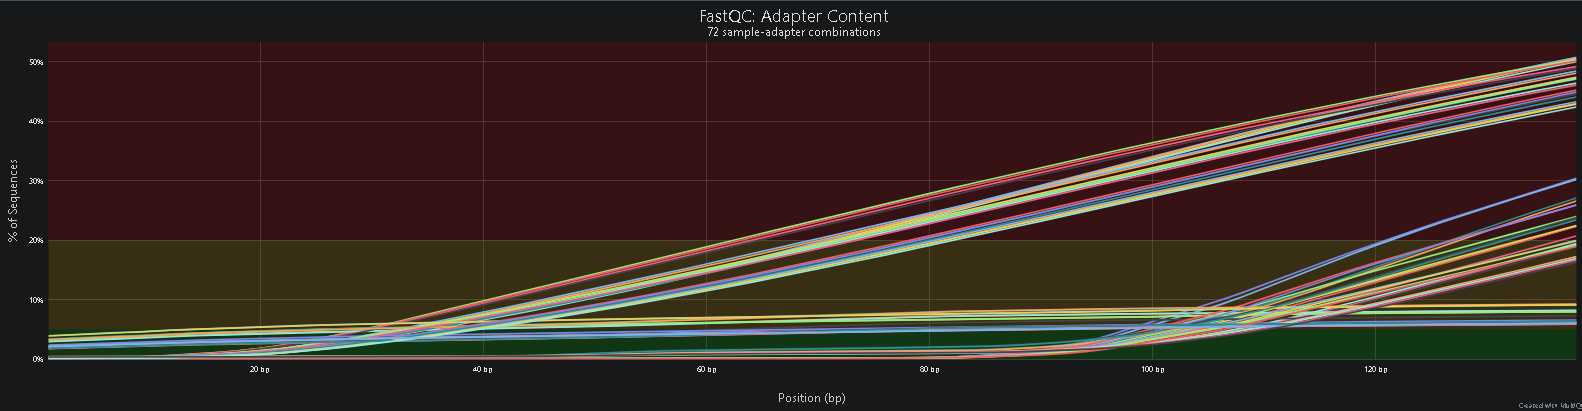
\includegraphics[keepaspectratio,alt={MultiQC plot de los datos crudos en la presencia de adaptadores en las secuencias}]{../results/QC/fastqc_adapter_content_plot_raw_data.png}}

}

\caption{Raw\_data\_adapters}

\end{figure}%

\begin{figure}[H]

{\centering \pandocbounded{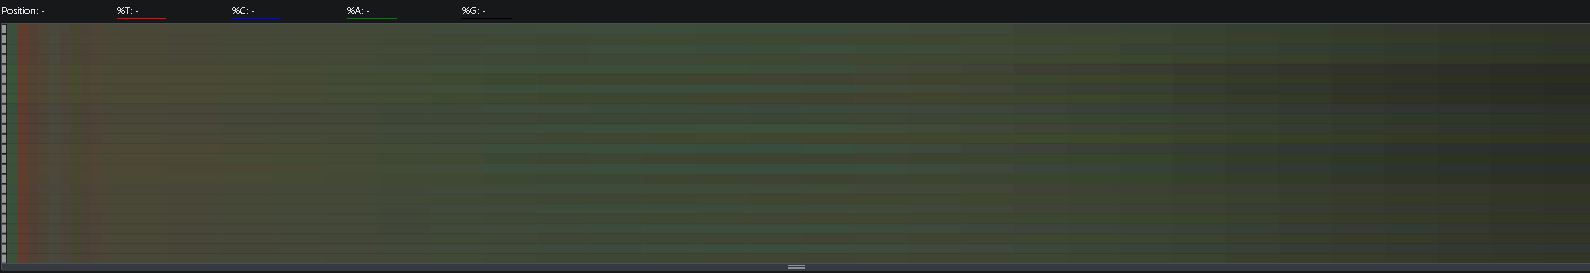
\includegraphics[keepaspectratio,alt={MultiQC plot de los datos crudos en relación a la calidad de las bases por posición}]{../results/QC/fastqc_per_base_sequence_content_plot_raw_data.png}}

}

\caption{Raw\_data\_base\_content}

\end{figure}%

\begin{figure}[H]

{\centering \pandocbounded{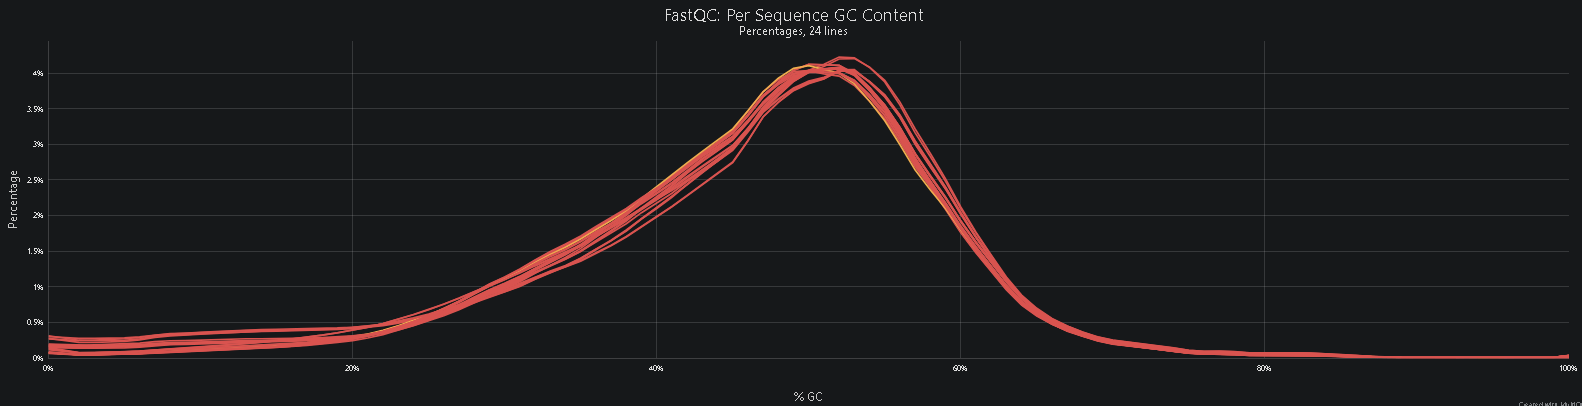
\includegraphics[keepaspectratio,alt={MultiQC plot de los datos crudos sobre el porcentaje de GC en las secuencias}]{../results/QC/fastqc_per_sequence_gc_content_plot_raw_data.png}}

}

\caption{Raw\_data\_gc\_content}

\end{figure}%

\begin{figure}[H]

{\centering \pandocbounded{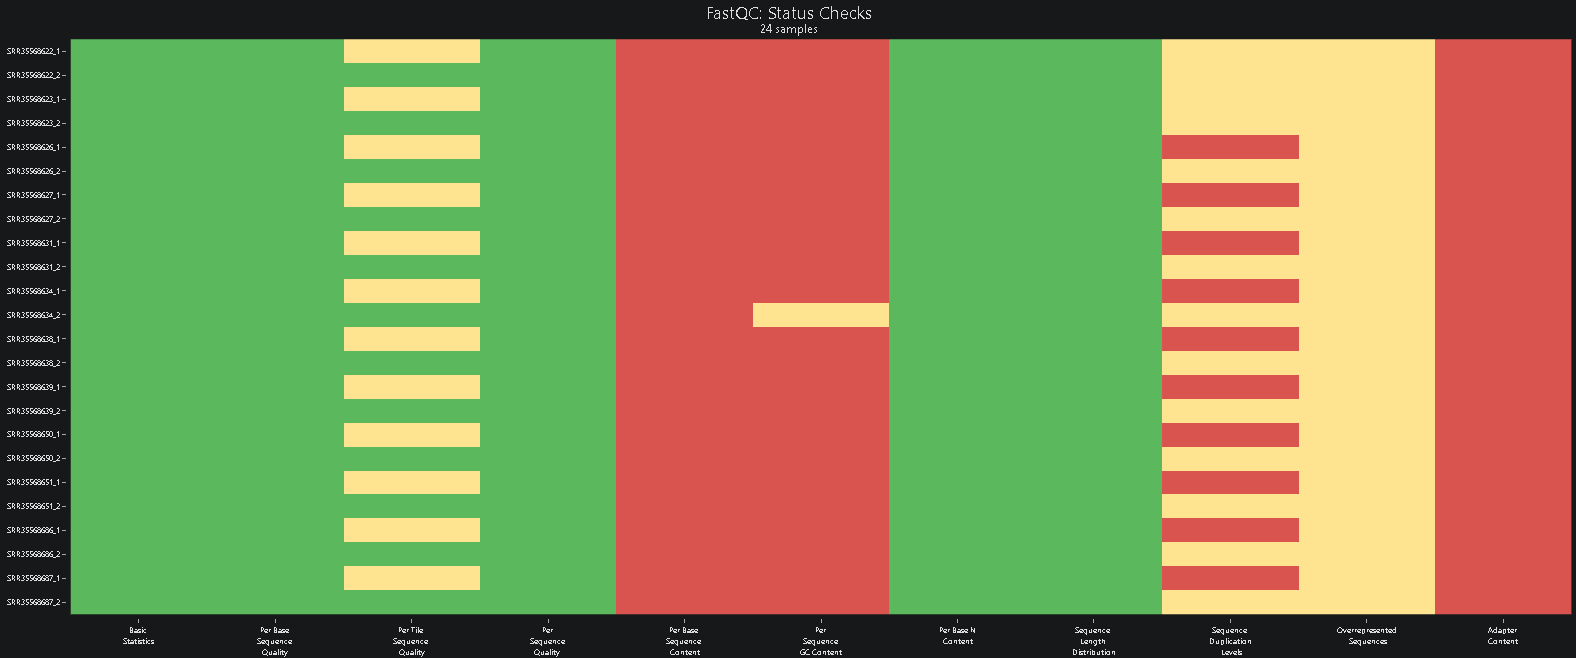
\includegraphics[keepaspectratio,alt={MultiQC heatmap estadisticas de control de calidad generales}]{../results/QC/fastqc-status-check-heatmap_raw_data.png}}

}

\caption{Raw\_data\_multi\_heatmap}

\end{figure}%

\subsubsection{Clean data}\label{clean-data}

\begin{figure}[H]

{\centering \pandocbounded{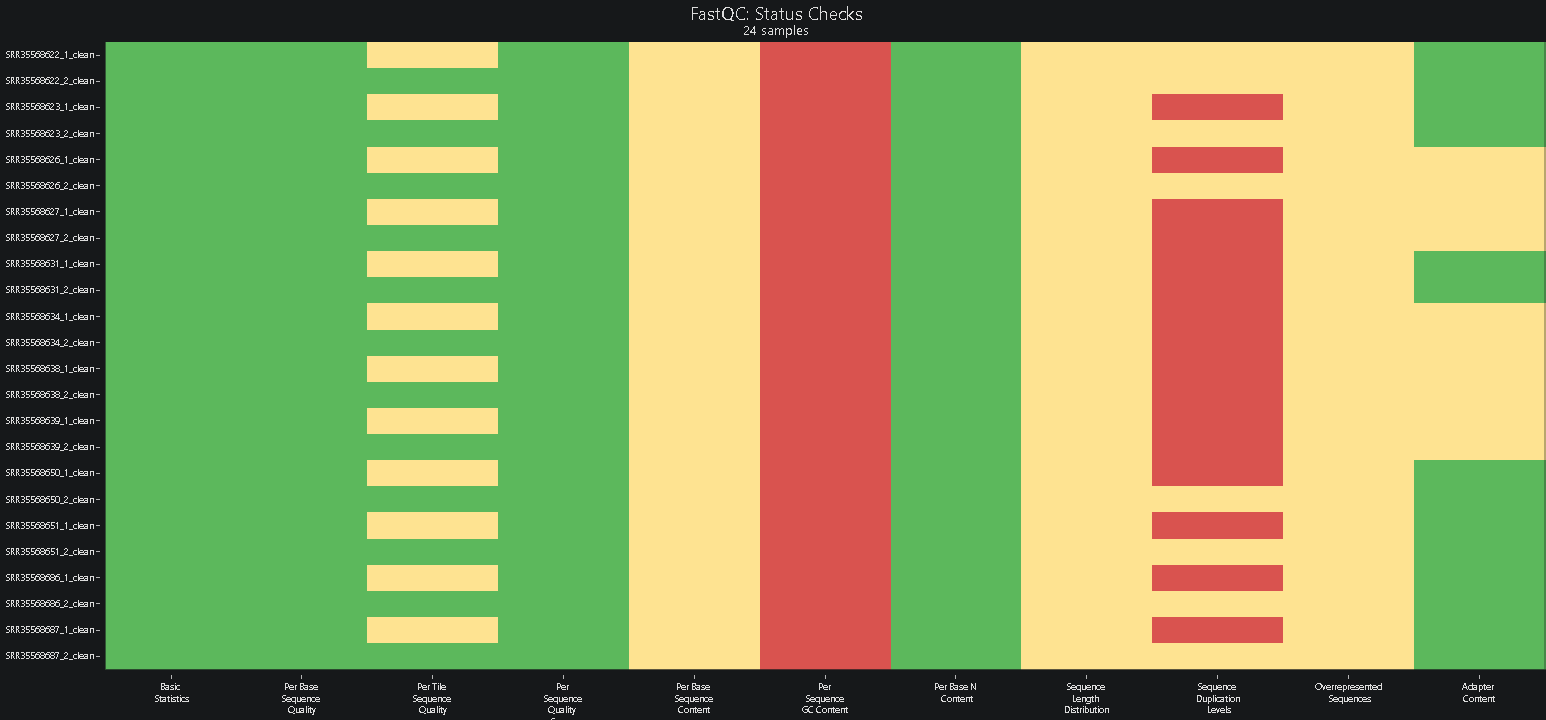
\includegraphics[keepaspectratio,alt={MultiQC heatmap estadisticas de control de calidad generales despues de la limpieza}]{../results/QC/fastqc-status-check-heatmap_clean_data.png}}

}

\caption{Clean\_data\_multi\_heatmap}

\end{figure}%

\subsection{DEA}\label{dea-1}

\subsubsection{Función multiploteo}\label{funciuxf3n-multiploteo}

\begin{Shaded}
\begin{Highlighting}[]
\NormalTok{\#| warning: false}
\NormalTok{\#| message: false}
\NormalTok{\#| eval: false}
\NormalTok{make\_multiplot \textless{}{-} function(plots\_list, name\_plot, colN = 4) \{}
\NormalTok{  \#revisar si la lista esta vacia}
\NormalTok{  if (length(plots\_list) \textless{} 1) \{}
\NormalTok{    return(NULL)}
\NormalTok{  \}}
\NormalTok{  \#eliminar los posibles null de las listas}
\NormalTok{  plots\_list \textless{}{-} Filter(Negate(is.null), plots\_list)}
\NormalTok{  \#cambiar el tipo de objeto de lo plots}

\NormalTok{  \#transformamos todos los plots a grob}
\NormalTok{  plots\_list \textless{}{-} lapply(plots\_list, function(p) \{}
\NormalTok{    \# ComplexHeatmap}
\NormalTok{    if (}
\NormalTok{      inherits(p, "Heatmap") ||}
\NormalTok{        inherits(p, "HeatmapList")}
\NormalTok{    ) \{}
\NormalTok{      return(}
\NormalTok{        grid::grid.grabExpr(}
\NormalTok{          ComplexHeatmap::draw(p)}
\NormalTok{        )}
\NormalTok{      )}
\NormalTok{    \}}
\NormalTok{    \# ggplot}
\NormalTok{    if (inherits(p, "ggplot")) \{}
\NormalTok{      return(ggplotGrob(p))}
\NormalTok{    \}}

\NormalTok{    \# ya es grob/gtable}
\NormalTok{    if (}
\NormalTok{      inherits(p, "grob") ||}
\NormalTok{        inherits(p, "gTree") ||}
\NormalTok{        inherits(p, "gtable")}
\NormalTok{    ) \{}
\NormalTok{      return(p)}
\NormalTok{    \}}
\NormalTok{    stop(}
\NormalTok{      "Tipo de plot no soportado: ",}
\NormalTok{      paste(class(p), collapse = ", ")}
\NormalTok{    )}
\NormalTok{  \})}

\NormalTok{  \#se hace el multiplot}
\NormalTok{  multi\_plot \textless{}{-} arrangeGrob(}
\NormalTok{    grobs = plots\_list,}
\NormalTok{    ncol = colN,}
\NormalTok{    top = textGrob(}
\NormalTok{      name\_plot,}
\NormalTok{      gp = gpar(fontsize = 16, fontface = "bold"),}
\NormalTok{      y = unit(0.5, "npc")}
\NormalTok{    )}
\NormalTok{  )}
\NormalTok{  return(multi\_plot)}
\NormalTok{\}}
\end{Highlighting}
\end{Shaded}

\subsubsection{edgeR hisat2}\label{edger-hisat2}

\begin{Shaded}
\begin{Highlighting}[]
\NormalTok{\#| warning: false}
\NormalTok{\#| message: false}
\NormalTok{\#Hacer el analisis de expresión diferencial con edegR}
\NormalTok{DE\_hisat$dea\_edgeR()}

\NormalTok{DE\_hisat$DEA\_edgeR$gen\_res}

\NormalTok{knitr::kable(}
\NormalTok{  head(DE\_hisat$DEA\_edgeR$gen\_res),}
\NormalTok{  format = "latex",}
\NormalTok{  booktabs = TRUE,}
\NormalTok{  caption = "Numero de genes Diferencialmente expresados hisat2 edgeR"}
\NormalTok{) \%\textgreater{}\%}
\NormalTok{  kable\_styling(latex\_options = c("scale\_down", "repeat\_header"))}

\NormalTok{\#multiploteo}
\NormalTok{DEA\_edgeR\_res = make\_multiplot(}
\NormalTok{  list(DE\_hisat$DEA\_edgeR$volcano\_plot, DE\_hisat$DEA\_edgeR$heatmap),}
\NormalTok{  "Resulatados hisat2 usando EdgeR",}
\NormalTok{  colN = 1}
\NormalTok{)}
\NormalTok{grid::grid.newpage()}
\NormalTok{grid::grid.draw(DEA\_edgeR\_res)}
\end{Highlighting}
\end{Shaded}

\subsubsection{STAR DEA}\label{star-dea}

\begin{Shaded}
\begin{Highlighting}[]
\NormalTok{\#| warning: false}
\NormalTok{\#| message: false}
\NormalTok{\#Assignamos un objeto al la lista con el nombre de la matriz correspondiente}
\NormalTok{DE\_star = DE\_obj$new(star\_count\_mtrx, metadata, "Astrocites\_eOH\_star\_pr")}

\NormalTok{\#pre{-}vizualization}
\NormalTok{DE\_star$pre\_vi("treatment", "sex")}

\NormalTok{pre\_vi\_plots = make\_multiplot(}
\NormalTok{  list(DE\_star$PCA\_p, DE\_star$Variance\_p),}
\NormalTok{  "Plots de previzualización matriz de conteos star",}
\NormalTok{  colN = 1}
\NormalTok{)}
\NormalTok{grid::grid.newpage()}
\NormalTok{grid::grid.draw(pre\_vi\_plots)}

\NormalTok{DE\_star$LFC = LFC}
\NormalTok{DE\_star$FDR = FDR}

\NormalTok{DE\_star$model = design\_add}
\NormalTok{DE\_star$contrast = contrast[, "condition\_con"]}

\NormalTok{DE\_star$dea\_deseq2()}
\NormalTok{DE\_star$dea\_edgeR()}

\NormalTok{over\_res = rbind(DE\_star$DEA\_edgeR$gen\_res, DE\_star$DEA\_DESeq2$gen\_res)}

\NormalTok{knitr::kable(}
\NormalTok{  head(over\_res),}
\NormalTok{  format = "latex",}
\NormalTok{  booktabs = TRUE,}
\NormalTok{  caption = "Numero de genes Diferencialmente expresados hisat2 edgeR"}
\NormalTok{) \%\textgreater{}\%}
\NormalTok{  kable\_styling(latex\_options = c("scale\_down", "repeat\_header"))}


\NormalTok{heatmap\_str\_ = DE\_star$DEA\_DESeq2$heatmap}
\NormalTok{volcano\_str = DE\_star$DEA\_DESeq2$volcano\_plot}

\NormalTok{DEA\_plots = make\_multiplot(}
\NormalTok{  list(}
\NormalTok{    DE\_star$DEA\_DESeq2$heatmap,}
\NormalTok{    DE\_star$DEA\_edgeR$heatmap,}
\NormalTok{    DE\_star$DEA\_DESeq2$volcano\_plot,}
\NormalTok{    DE\_star$DEA\_edgeR$volcano\_plot}
\NormalTok{  ),}
\NormalTok{  "Resultados DEA matriz STAR ",}
\NormalTok{  colN = 2}
\NormalTok{)}
\NormalTok{grid::grid.newpage()}
\NormalTok{grid::grid.draw(DEA\_plots)}
\end{Highlighting}
\end{Shaded}





\end{document}
